\documentclass{beamer}

\usepackage{xparse}
\usepackage{kotex}
\usepackage{graphicx}
\usepackage{minted}
\usepackage[export]{adjustbox}
\usepackage{textcomp}

\vfuzz=30pt

%%%%%%%%%%%%%%%%%%%%%
%  Beamer Settings  %
%%%%%%%%%%%%%%%%%%%%%
\usetheme[numbering=fraction]{metropolis}
\usecolortheme{rose}
\useoutertheme[subsection=false]{miniframes}

\setbeamertemplate{itemize item}[square]
\setbeamertemplate{itemize subitem}[triangle]
\setbeamertemplate{itemize subsubitem}[circle]

%%%%%%%%%%%%%%%%%%%
%  Font Settings  %
%%%%%%%%%%%%%%%%%%%
\usepackage[factor=500]{microtype}

\usepackage[mathrm=sym]{unicode-math}

\setsansfont{Roboto}[
  BoldFont = *-Medium,
  BoldItalicFont = *-MediumItalic
]
\setmonofont{Inconsolata}
\setsanshangulfont{NanumGothic}[AutoFakeSlant=0.18]

%%%%%%%%%%%%%%%%%%%%%
%  Minted Settings  %
%%%%%%%%%%%%%%%%%%%%%
\renewcommand\theFancyVerbLine{\textsf{\tiny\arabic{FancyVerbLine}}}

\newminted{latex}{
  escapeinside=||,
  mathescape,
  autogobble,
  linenos,
  breaklines,
  numbersep=5pt,
  frame=single,
  fontsize=\scriptsize}
\newmintinline[ltxverb]{latex}{escapeinside=||}

%%%%%%%%%%%%%%%%%%%%%%%
% Custom Settings  %
%%%%%%%%%%%%%%%%%%%%%%%
\def\tbs{\textbackslash}

\newcommand*{\numberofpages}[1]{%
  \the\XeTeXpdfpagecount"#1" %
}

%%%%%%%%%%%%%%%%%%%%%%%
%  Document Settings  %
%%%%%%%%%%%%%%%%%%%%%%%

\title{%
  {\large Memoir로 해보는 Book Design}\\
  Chapter Style
}

\author{이재호}
\institute{서울대학교 전기$\cdot$정보공학부/KTUG}
\date{2019년 11월 16일}

%%%%%%%%%%%%%%
%  Document  %
%%%%%%%%%%%%%%
\begin{document}

\maketitle

\section{Overview}

\begin{frame}[fragile]{Memoir 챕터}
  \begin{columns}
    \begin{column}{0.6\textwidth}
      Memoir의 기본 챕터의 모양\vspace*{\baselineskip}

      \pause
      \begin{latexcode}
        \documentclass[a4paper]{memoir}
        \usepackage{lipsum}
        \begin{document}
        \chapter{Foo}
        \lipsum[1-4]
        \end{document}
      \end{latexcode}
    \end{column}
    \begin{column}{0.4\textwidth}
      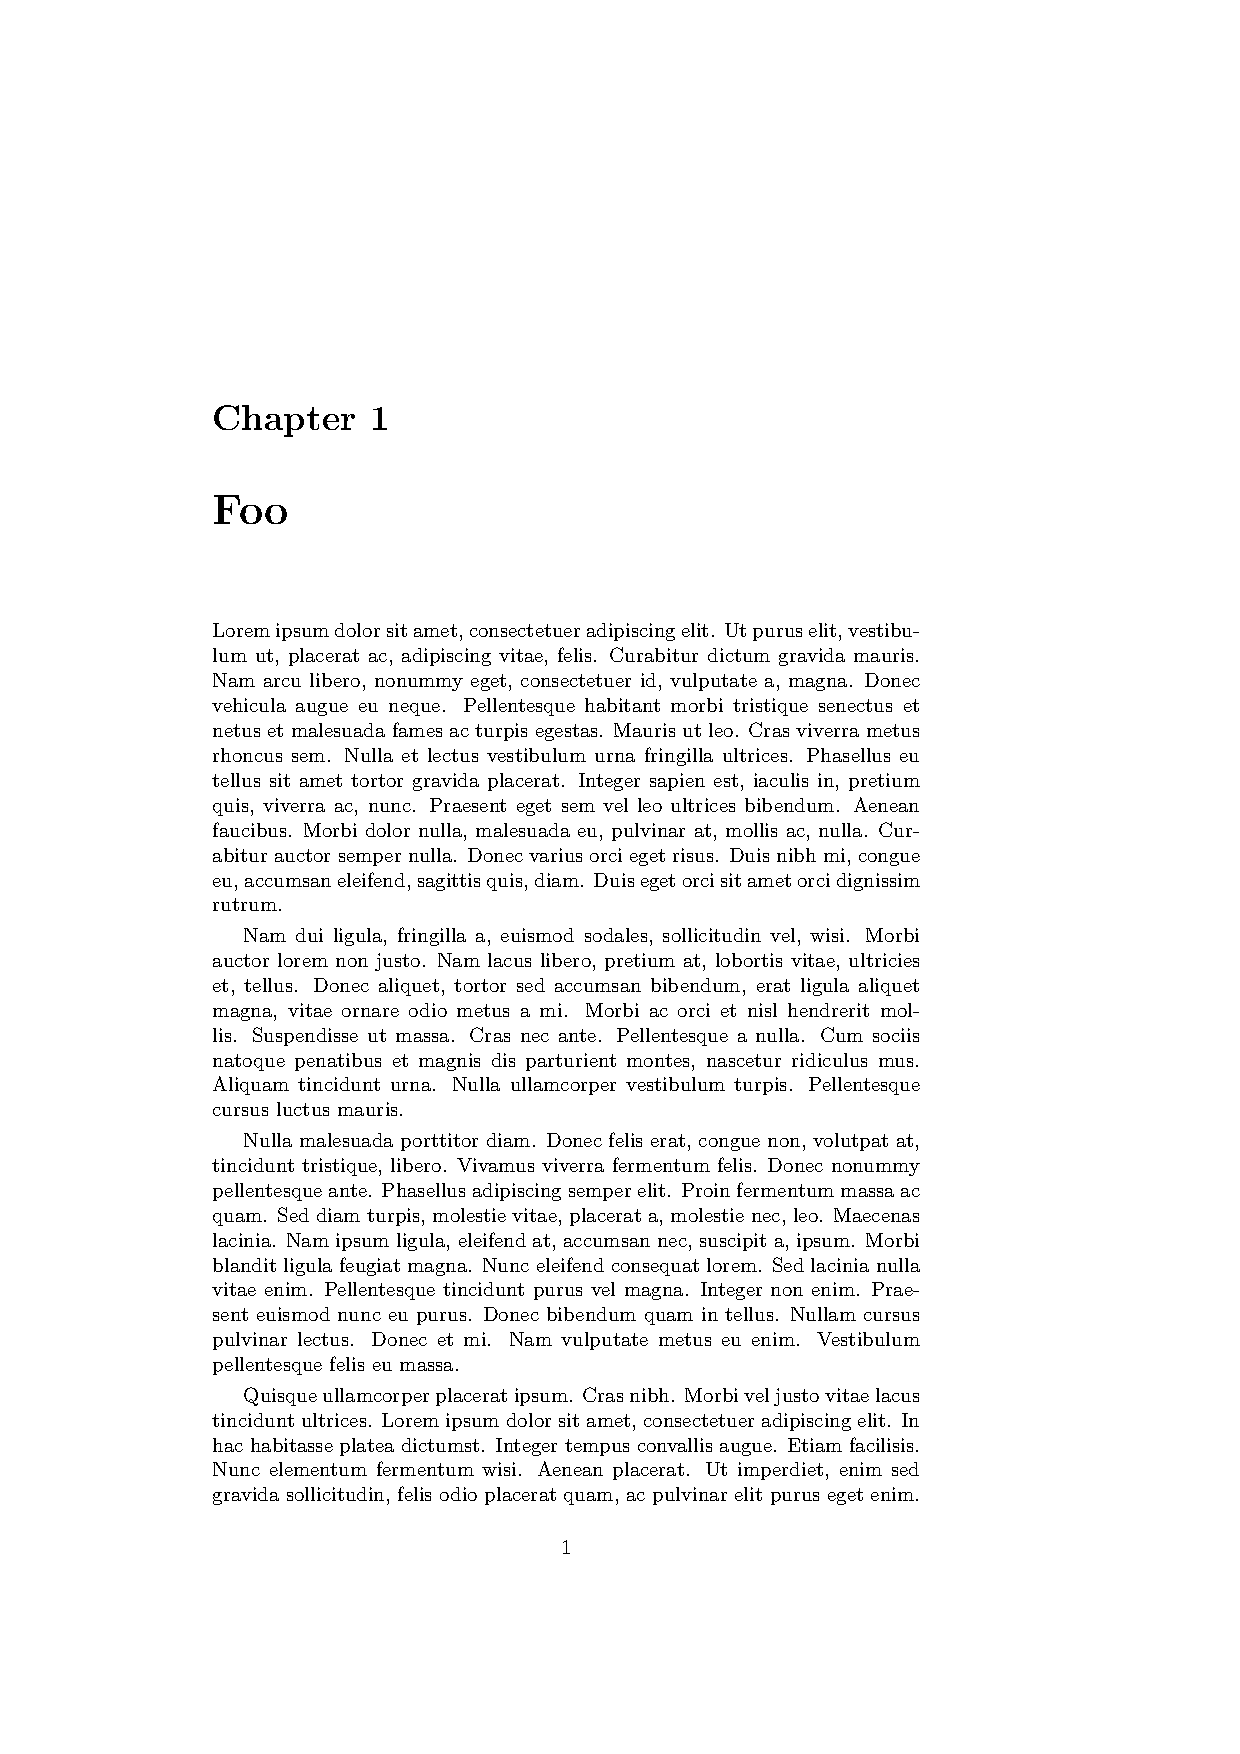
\includegraphics[frame,page=1,width=\linewidth]{examples/chapterheadstart}
    \end{column}
  \end{columns}
  \pause
  입맛에 맞게 꾸미고 싶다면?
\end{frame}

\begin{frame}[fragile]{예시}
  \ExplSyntaxOn
  \int_set:Nn \l_tmpa_int
    {
      \numberofpages { examples/showcases.pdf } / 2
    }
  \begin{columns}
    \begin{column}{0.43\textwidth}
      \begin{overprint}
        \int_step_inline:nn { \l_tmpa_int }
          {
            \onslide<#1>
            \includegraphics[frame,
                             page={ \int_eval:n { #1 * 2 - 1 } },
                             width=\linewidth]{examples/showcases}
          }
      \end{overprint}
    \end{column}
    \begin{column}{0.43\textwidth}
      \begin{overprint}
        \int_step_inline:nn { \l_tmpa_int }
          {
            \onslide<#1>
            \includegraphics[frame,
                             page={ \int_eval:n { #1 * 2 } },
                             width=\linewidth]{examples/showcases}
          }
      \end{overprint}
    \end{column}
  \end{columns}
  \ExplSyntaxOff
\end{frame}

\begin{frame}[fragile]{\texttt{\textbackslash chapter}가 하는 일}
  Memoir에서 챕터 모양을 바꾸기 위해서는 \ltxverb/\chapterstyle{|<style>|}/ 사용

  \pause
  일반적으로 \LaTeX에서는 \ltxverb/\@makechapterhead/로 \ltxverb/\chapter/의
  서식을 지정, \ltxverb/\@makeschapterhead/로 \ltxverb/\chapter*/의 서식을 지정

  \pause
  Memoir에서는 대략...
  \begin{columns}[T]
    \begin{column}{0.5\textwidth}
      \begin{latexcode}
        % \chapter with secnumdepth $\geq$ 0
        \chapterheadstart
        \printchaptername \chapternamenum \printchapternum
        \afterchapternum
        \printchaptertitle{The title}
        \afterchaptertitle
      \end{latexcode}
    \end{column}

    \begin{column}{0.5\textwidth}
      \begin{latexcode}
        % \chapter* with secnumdepth < 0
        \chapterheadstart
        \printchapternonum
        \printchaptertitle{The title}
        \afterchaptertitle
      \end{latexcode}
    \end{column}
  \end{columns}
\end{frame}

\begin{frame}[fragile]{\texttt{\textbackslash chapterstyle}이 하는 일}
  매 chapter style 마다, 다음과 같은 매크로들이 초기화된다:
  \begin{latexcode}
    \renewcommand\chapterheadstart{\vspace*{\beforechapskip}}
    \renewcommand\printchaptername{\chapnamefont \@chapapp}
    \renewcommand\chapternamenum{\space}
    \renewcommand\printchapternum{\chapnumfont \thechapter}
    \renewcommand\afterchapternum{\par\nobreak\vskip \midchapskip}
    \renewcommand\printchapternonum{}
    \renewcommand\printchaptertitle[1]{\chaptitlefont #1}
    \renewcommand\afterchaptertitle{\par\nobreak\vskip \afterchapskip}
  \end{latexcode}

  \pause
  마지막으로, \ltxverb/\makechapterstyle{|<style>|}{|<code>|}/를 통해 새로운
  chapter style을 정의할 수 있다.

  이를 사용하려면, \ltxverb/\chapterstyle{|<name>|}/을 사용한다.
\end{frame}


\section{명령어 분석}

\begin{frame}[fragile]
  {\texttt{\tbs openright}, \texttt{\tbs openleft}, \texttt{\tbs openany} 분석}
  \begin{description}
    \item[openright] 챕터 헤딩이 직후 우측 페이지에 위치한다.
    \item[openleft] 챕터 헤딩이 직후 좌측 페이지에 위치한다.
    \item[openany] 챕터 헤딩이 직후 페이지에 위치한다.
  \end{description}

  또한 \ltxverb/\openright/와 같이 문서 아무 곳에서 사용하면 설정이 바뀐다.

  \pause
  이는 다음과 같은 일을 하도록 정의되어 있다:
  \begin{latexcode}
    \newcommand{\openright}{\@openrighttrue\@openleftfalse%
      \gdef\clearforchapter{\cleartorecto}}
    \newcommand{\openany}{\@openrightfalse\@openleftfalse%
      \gdef\clearforchapter{\clearpage}}
    \newcommand{\openleft}{\@openlefttrue
      \gdef\clearforchapter{\cleartoverso}}
  \end{latexcode}
\end{frame}

\begin{frame}[fragile]{\texttt{\tbs clearforchapter} 분석}
  직전에 소개된 \ltxverb/\openright/, \ltxverb/\openleft/, \ltxverb/\openany/에
  의해 설정된다.

  만약 이를 새로 정의한다면 챕터가 시작되기 직전에 해야하는 작업을 수행할 수
  있다.
\end{frame}

\begin{frame}[fragile]{\texttt{\tbs clearforchapter} 예시}
  \begin{latexcode}
    \renewcommand*{\clearforchapter}{}
  \end{latexcode}

  \begin{columns}
    \begin{column}{0.4\textwidth}
      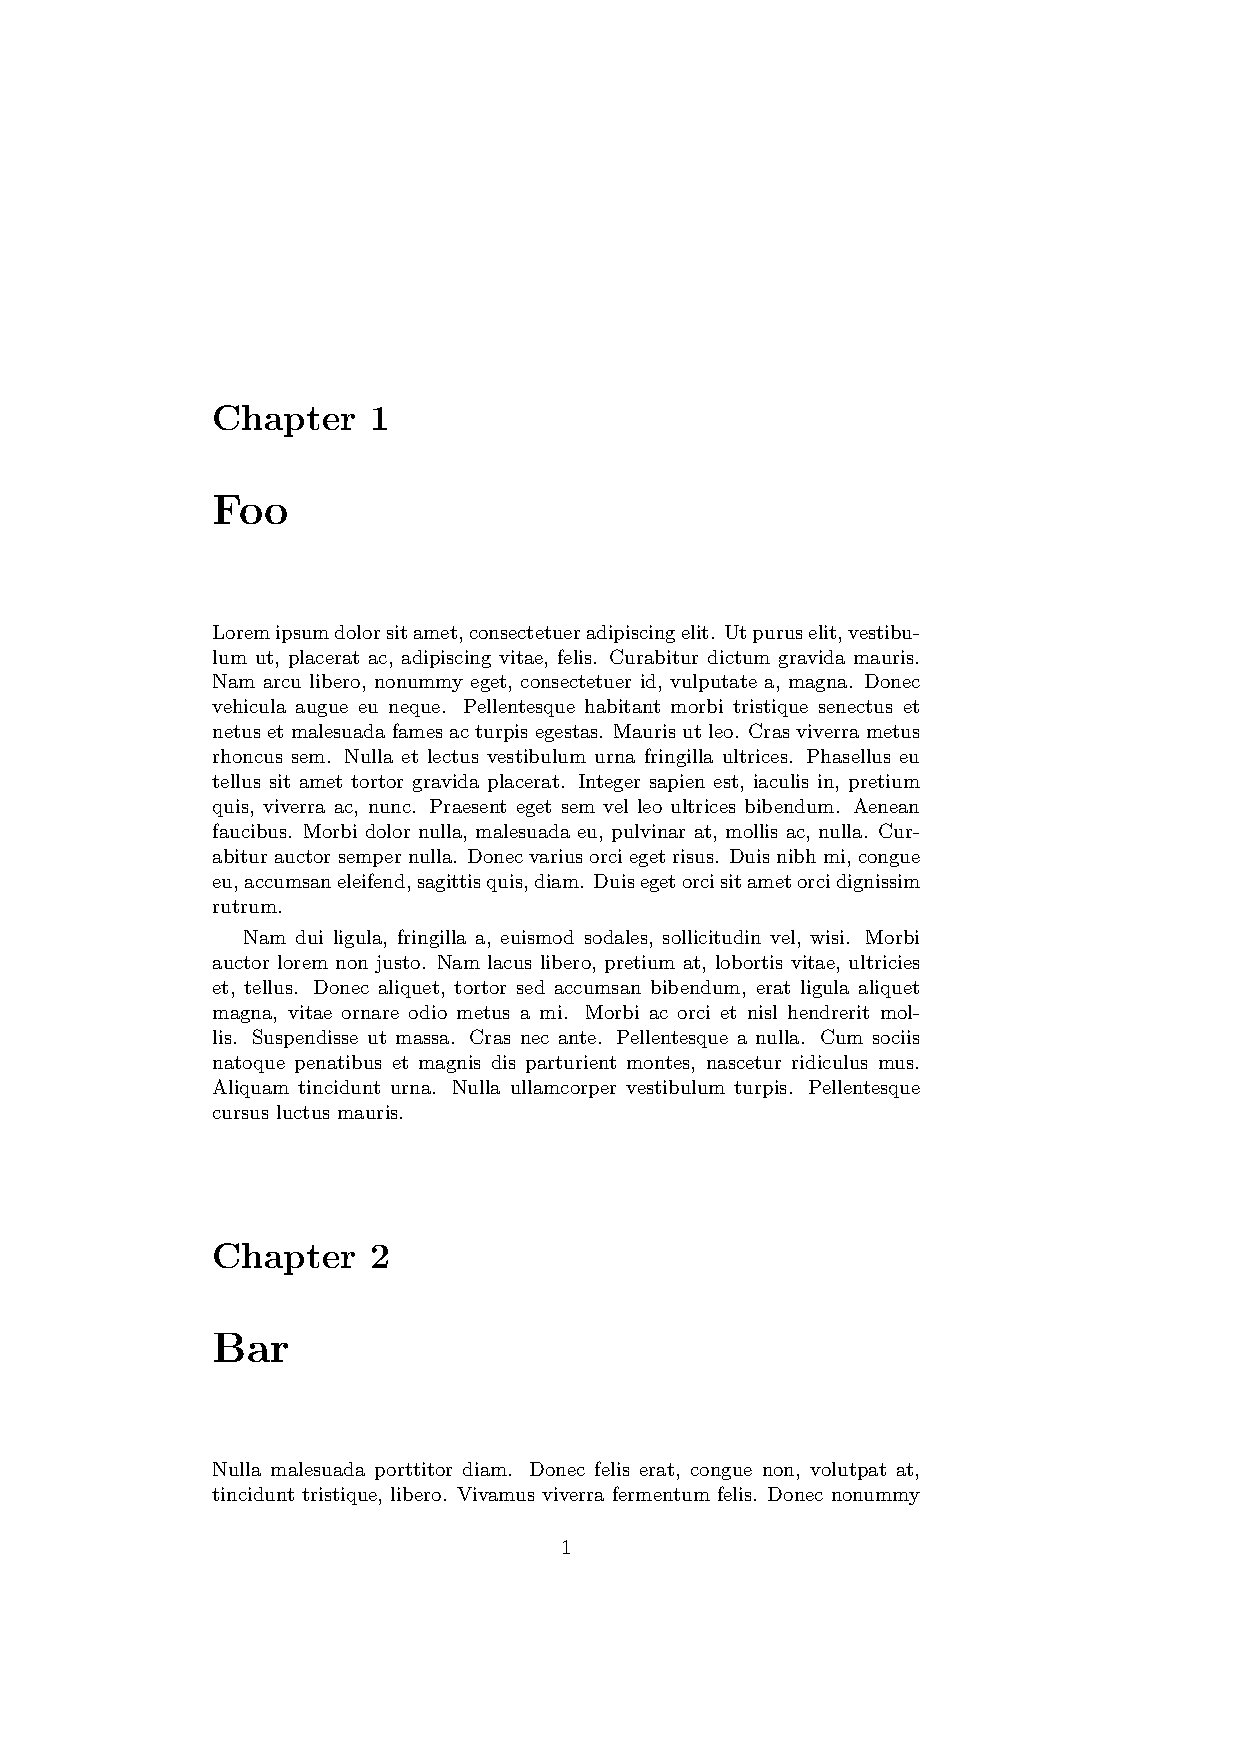
\includegraphics[frame,page=1,width=\linewidth]{examples/clearforchapter}
    \end{column}
    \begin{column}{0.4\textwidth}
      \includegraphics[frame,page=2,width=\linewidth]{examples/clearforchapter}
    \end{column}
  \end{columns}
\end{frame}

\begin{frame}[fragile]{\texttt{\tbs memendofchapterhook} 분석}
  \ltxverb/\clearforchapter/가 챕터 시작 직전에 실행된다면,
  \ltxverb/\memendofchapterhook/은 챕터의 맨 끝에서 실행된다.

  기본적으로는 아무것도 하지 않도록 정의되어 있다.
\end{frame}

\begin{frame}[fragile]{\texttt{\tbs memendofchapterhook} 예시}
  \begin{columns}
    \begin{column}{0.6\textwidth}
      \begin{latexcode}
        % \usepackage{amssymb}
        \renewcommand*{\clearforchapter}{}
        \renewcommand{\memendofchapterhook}{%
          \begin{center}
            $\lozenge\lozenge\lozenge$
          \end{center}}
      \end{latexcode}
    \end{column}

    \begin{column}{0.4\textwidth}
      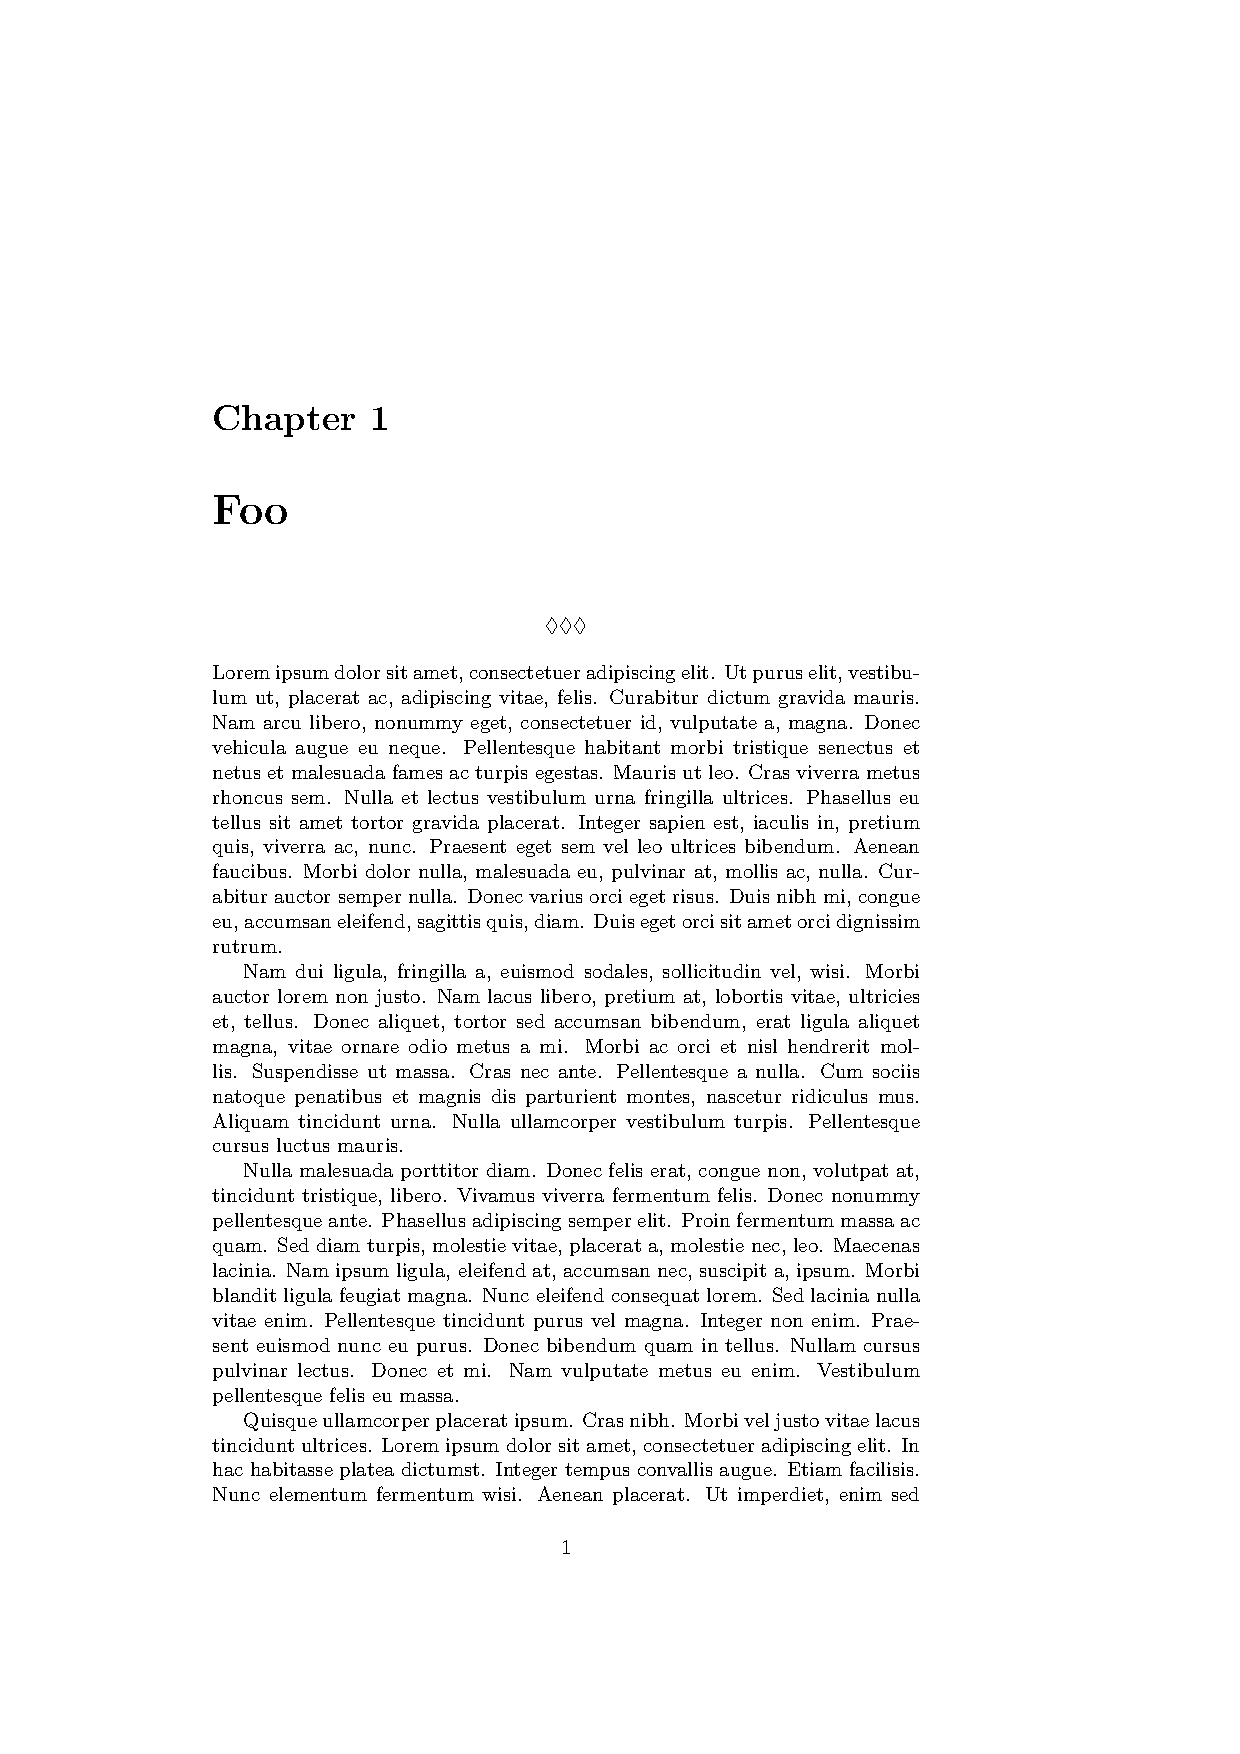
\includegraphics[frame,page=1,width=\linewidth]{examples/memendofchapterhook}
    \end{column}
  \end{columns}
\end{frame}

\begin{frame}[fragile]
  {\texttt{\tbs chapterheadstart}와 \texttt{\tbs beforechapskip} 분석}
  \ltxverb/\chapterheadstart/은 챕터 제목과 번호를 출력하기 직전에 실행되며,
  기본적으로는 50pt로 설정되어 있는 \ltxverb/\beforechapskip/을 출력한다.
\end{frame}

\begin{frame}[fragile]
  {\texttt{\tbs chapterheadstart}와 \texttt{\tbs beforechapskip} 예시}
  \begin{overprint}
    \onslide<1>
    \begin{columns}
      \begin{column}{0.5\textwidth}
        \begin{latexcode}
          \setlength\beforechapskip{50pt}
        \end{latexcode}
        \begin{center}
          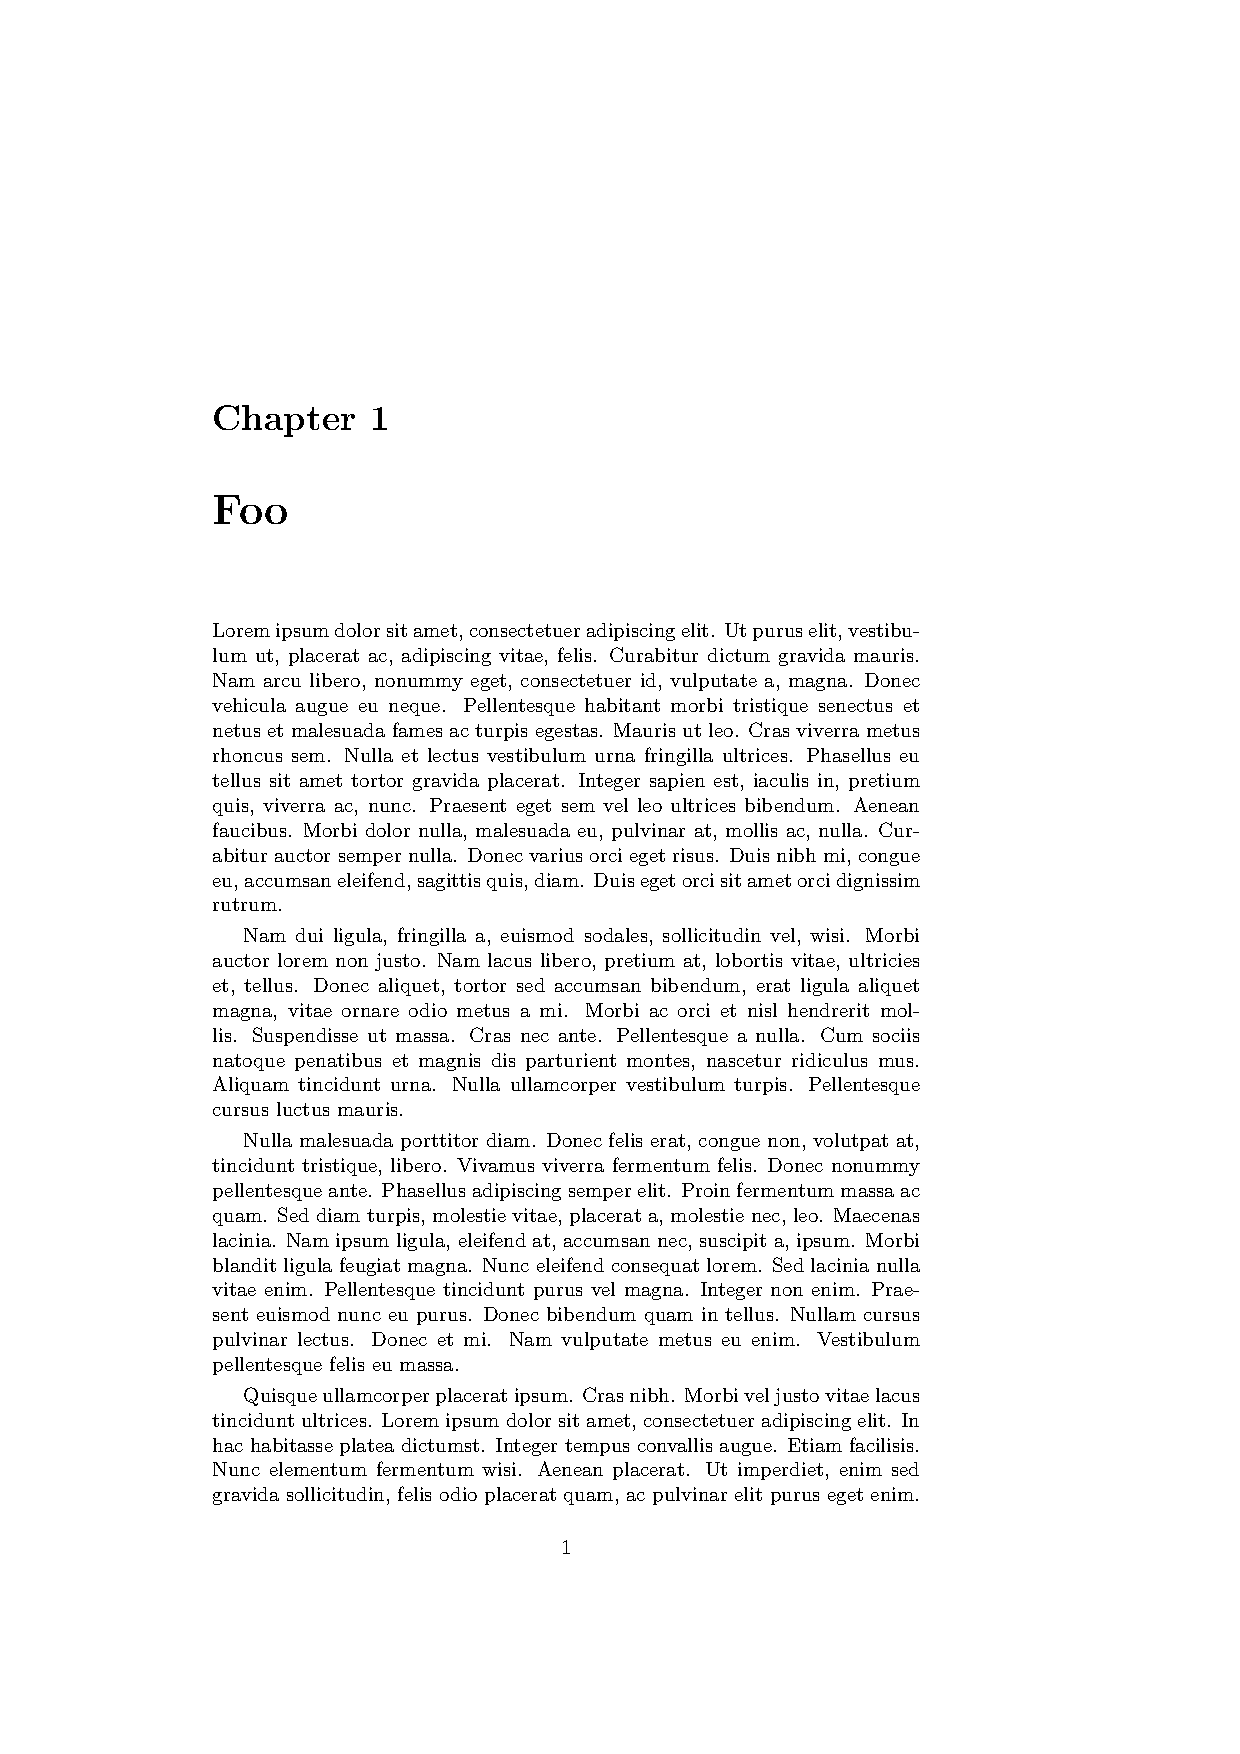
\includegraphics[frame,page=1,width=0.8\linewidth]{examples/chapterheadstart}
        \end{center}
      \end{column}

      \begin{column}{0.5\textwidth}
        \begin{minted}[mathescape,
                       autogobble,
                       linenos,
                       numbersep=5pt,
                       frame=single,
                       fontsize=\scriptsize]{latex}
          \setlength\beforechapskip{-\baselineskip}
        \end{minted}
        \begin{center}
          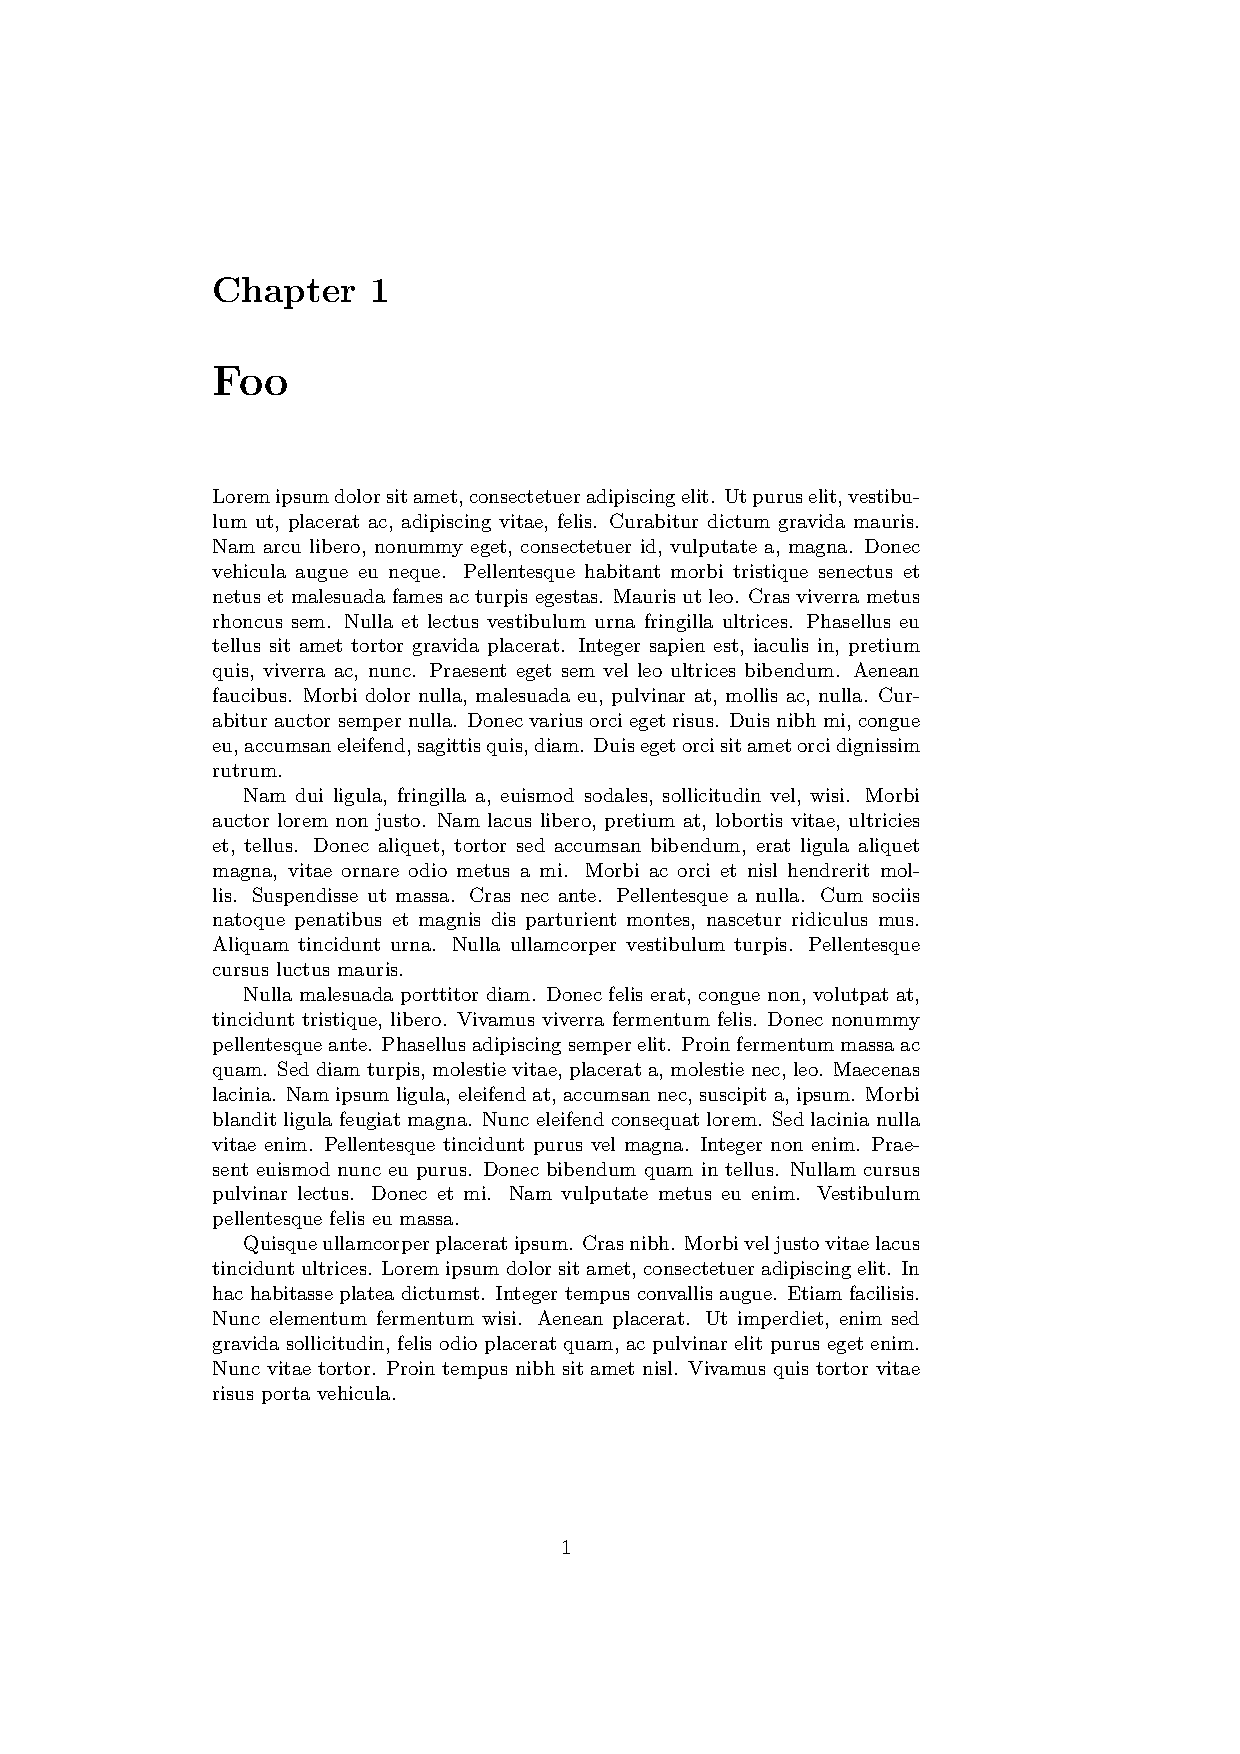
\includegraphics[frame,page=1,width=0.8\linewidth]{examples/chapterheadstart-2}
        \end{center}
      \end{column}
    \end{columns}

    \onslide<2>
    \begin{columns}
      \begin{column}{0.5\textwidth}
        \begin{latexcode}
          \setlength\beforechapskip{50pt}
        \end{latexcode}
        \begin{center}
          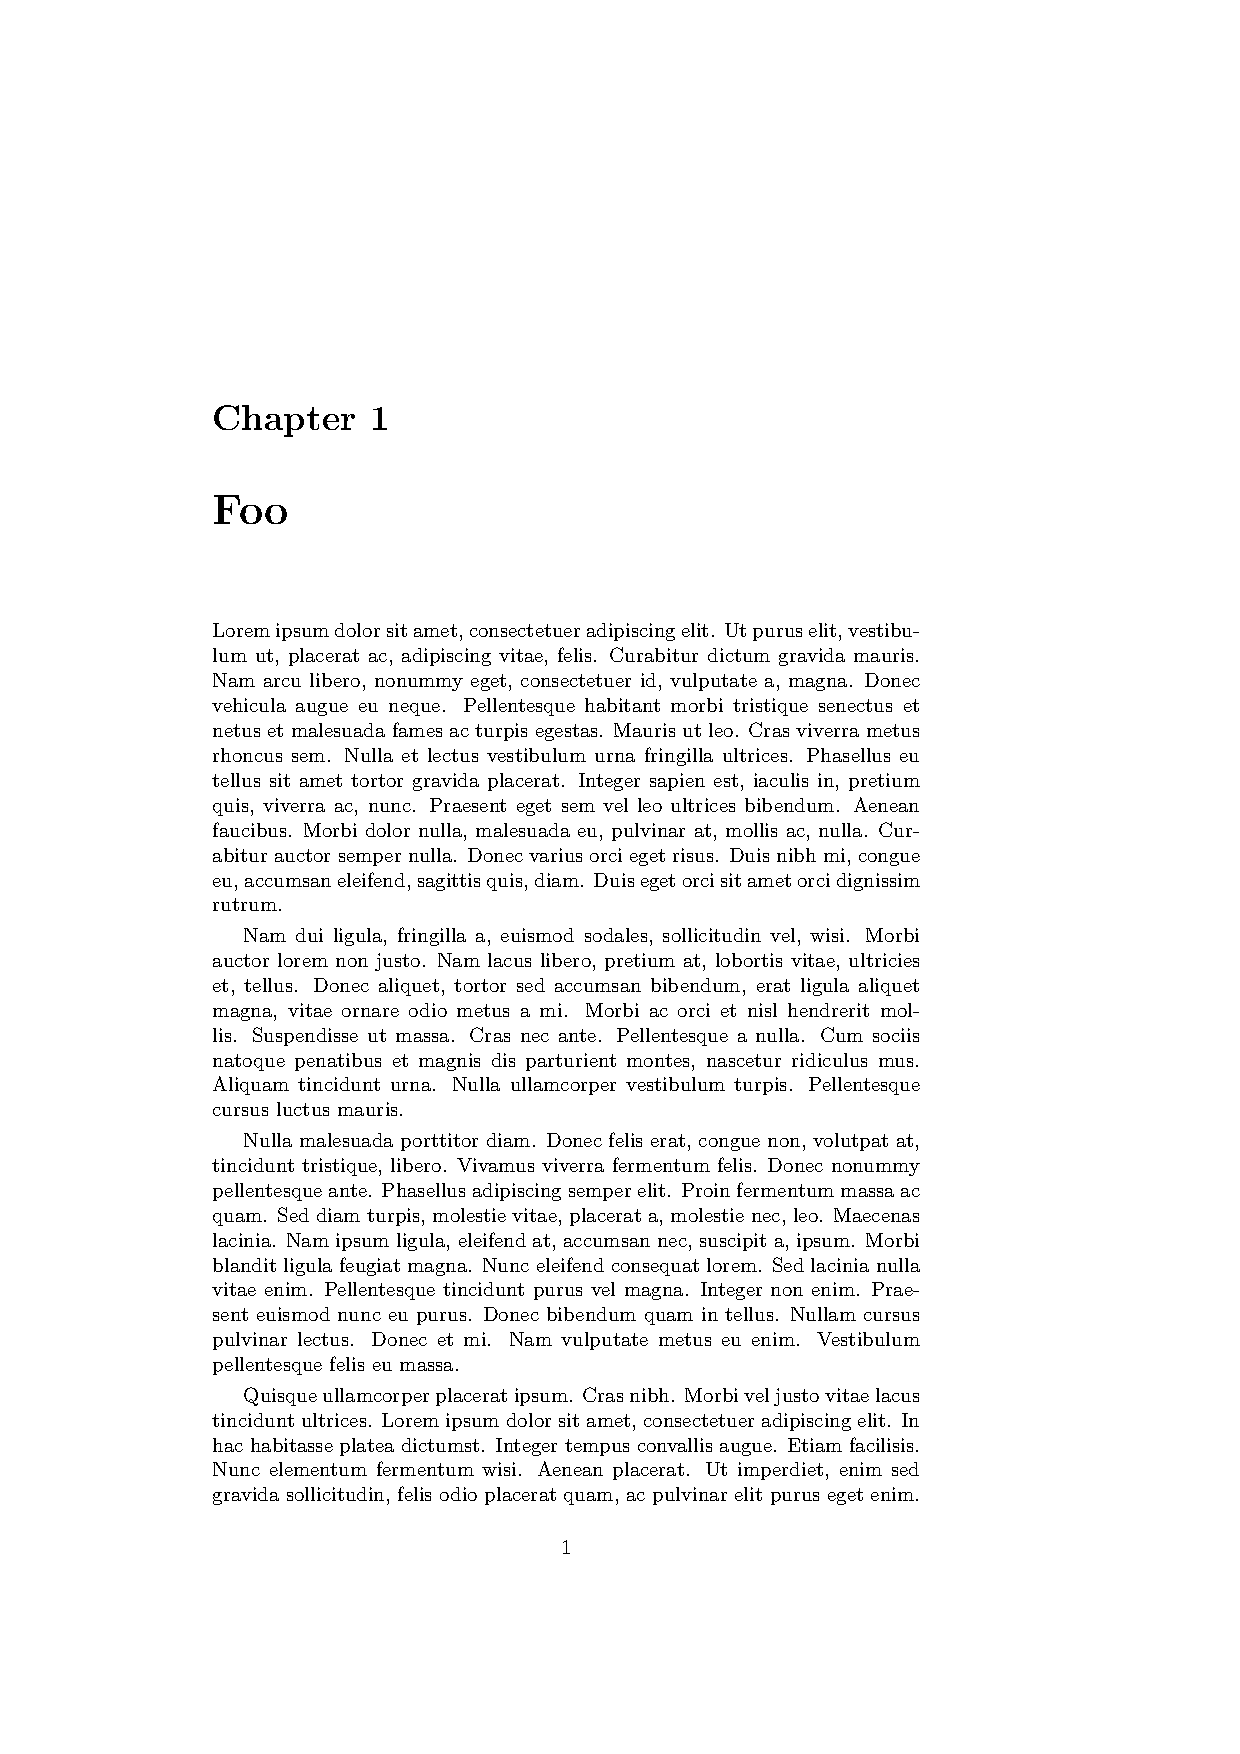
\includegraphics[frame,page=1,width=0.8\linewidth]{examples/chapterheadstart}
        \end{center}
      \end{column}

      \begin{column}{0.5\textwidth}
        \begin{latexcode}
          \renewcommand*{\chapterheadstart}{}
        \end{latexcode}
        \begin{center}
          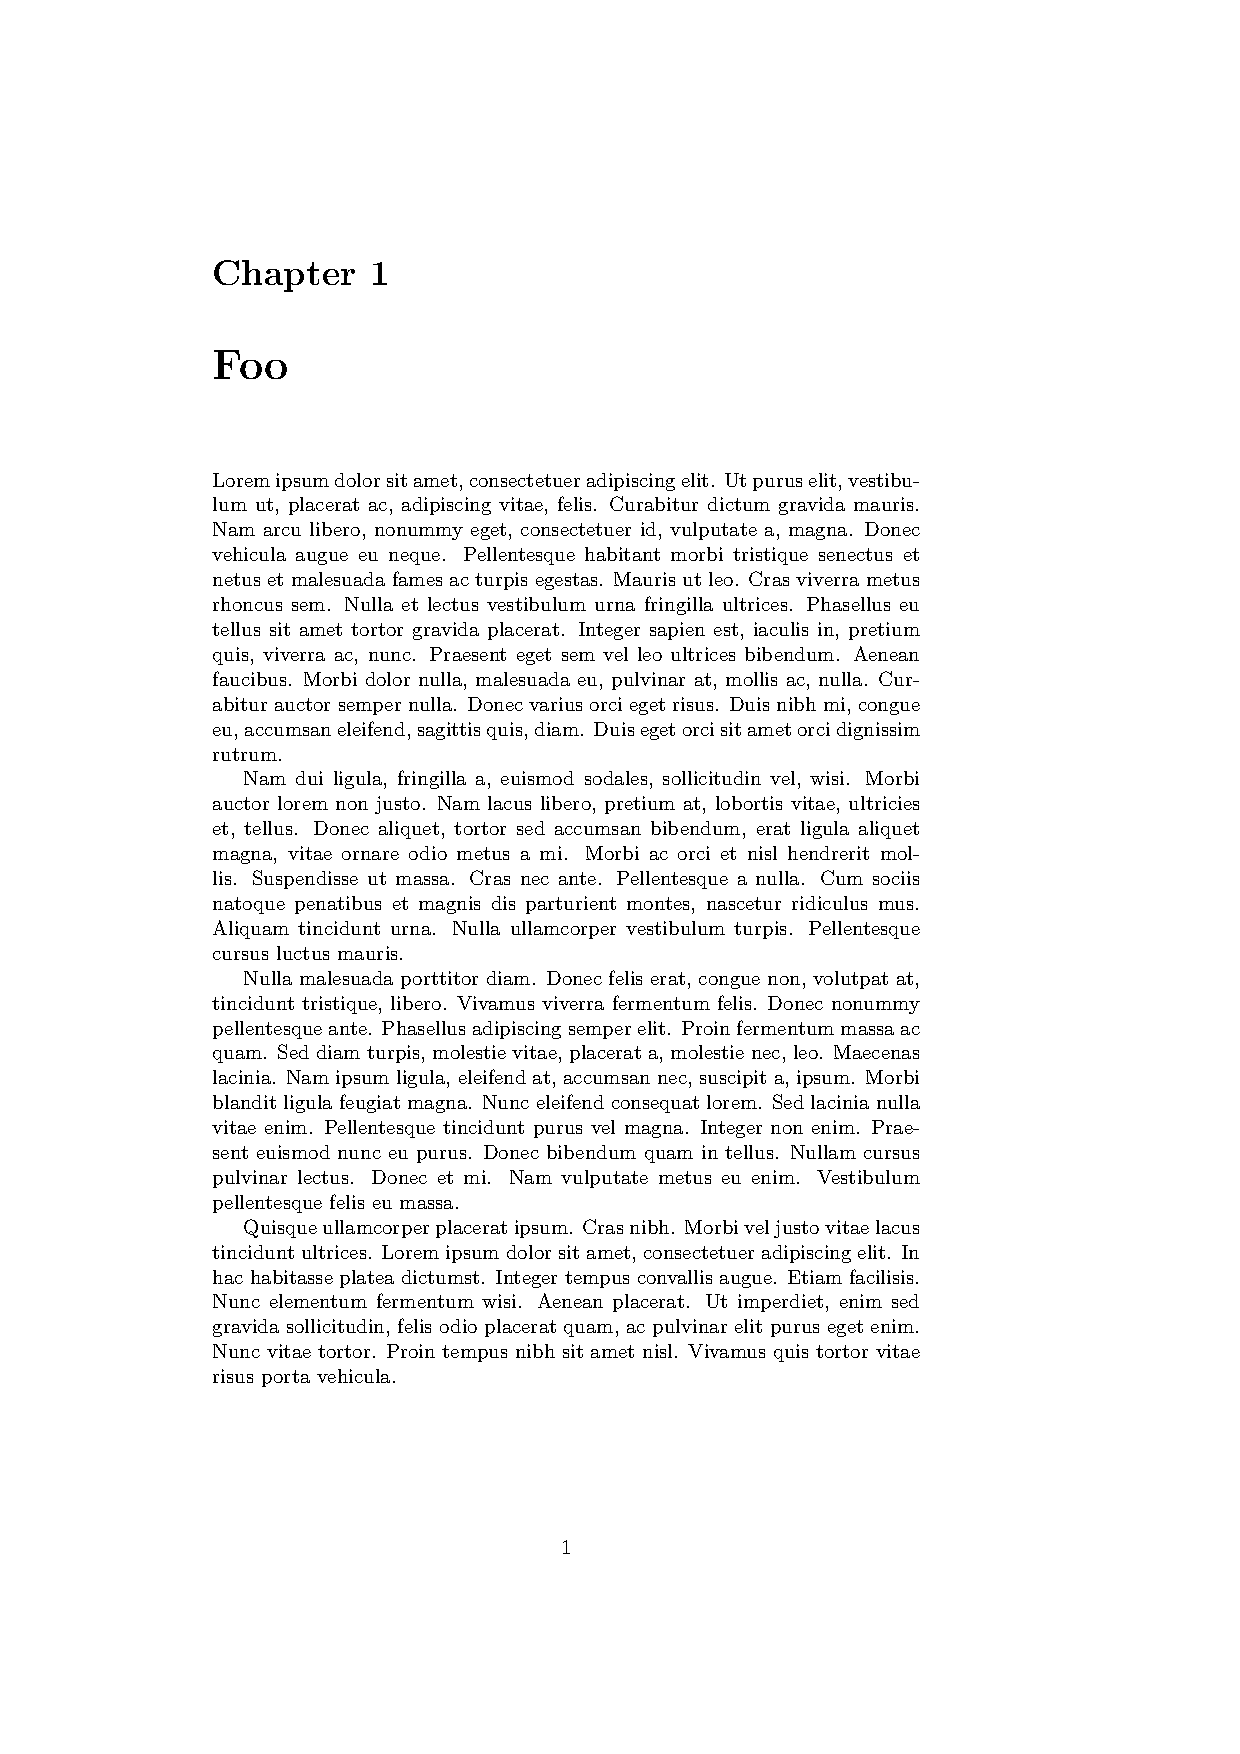
\includegraphics[frame,page=1,width=0.8\linewidth]{examples/chapterheadstart-3}
        \end{center}
      \end{column}
    \end{columns}
  \end{overprint}
\end{frame}

\begin{frame}[fragile]
  {\texttt{\tbs afterchapternum}과 \texttt{\tbs midchapskip} 분석}
  \ltxverb/\afterchapternum/은 챕터 번호를 출력한 직후에 실행되며, 기본적으로는
  20pt로 설정되어 있는 \ltxverb/\midchapskip/을 출력한다.
\end{frame}

\begin{frame}[fragile]
  {\texttt{\tbs afterchapternum}과 \texttt{\tbs midchapskip} 예시}
  \begin{overprint}
    \onslide<1>
    \begin{columns}
      \begin{column}{0.5\textwidth}
        \begin{latexcode}
          \setlength\midchapskip{20pt}
        \end{latexcode}
        \begin{center}
          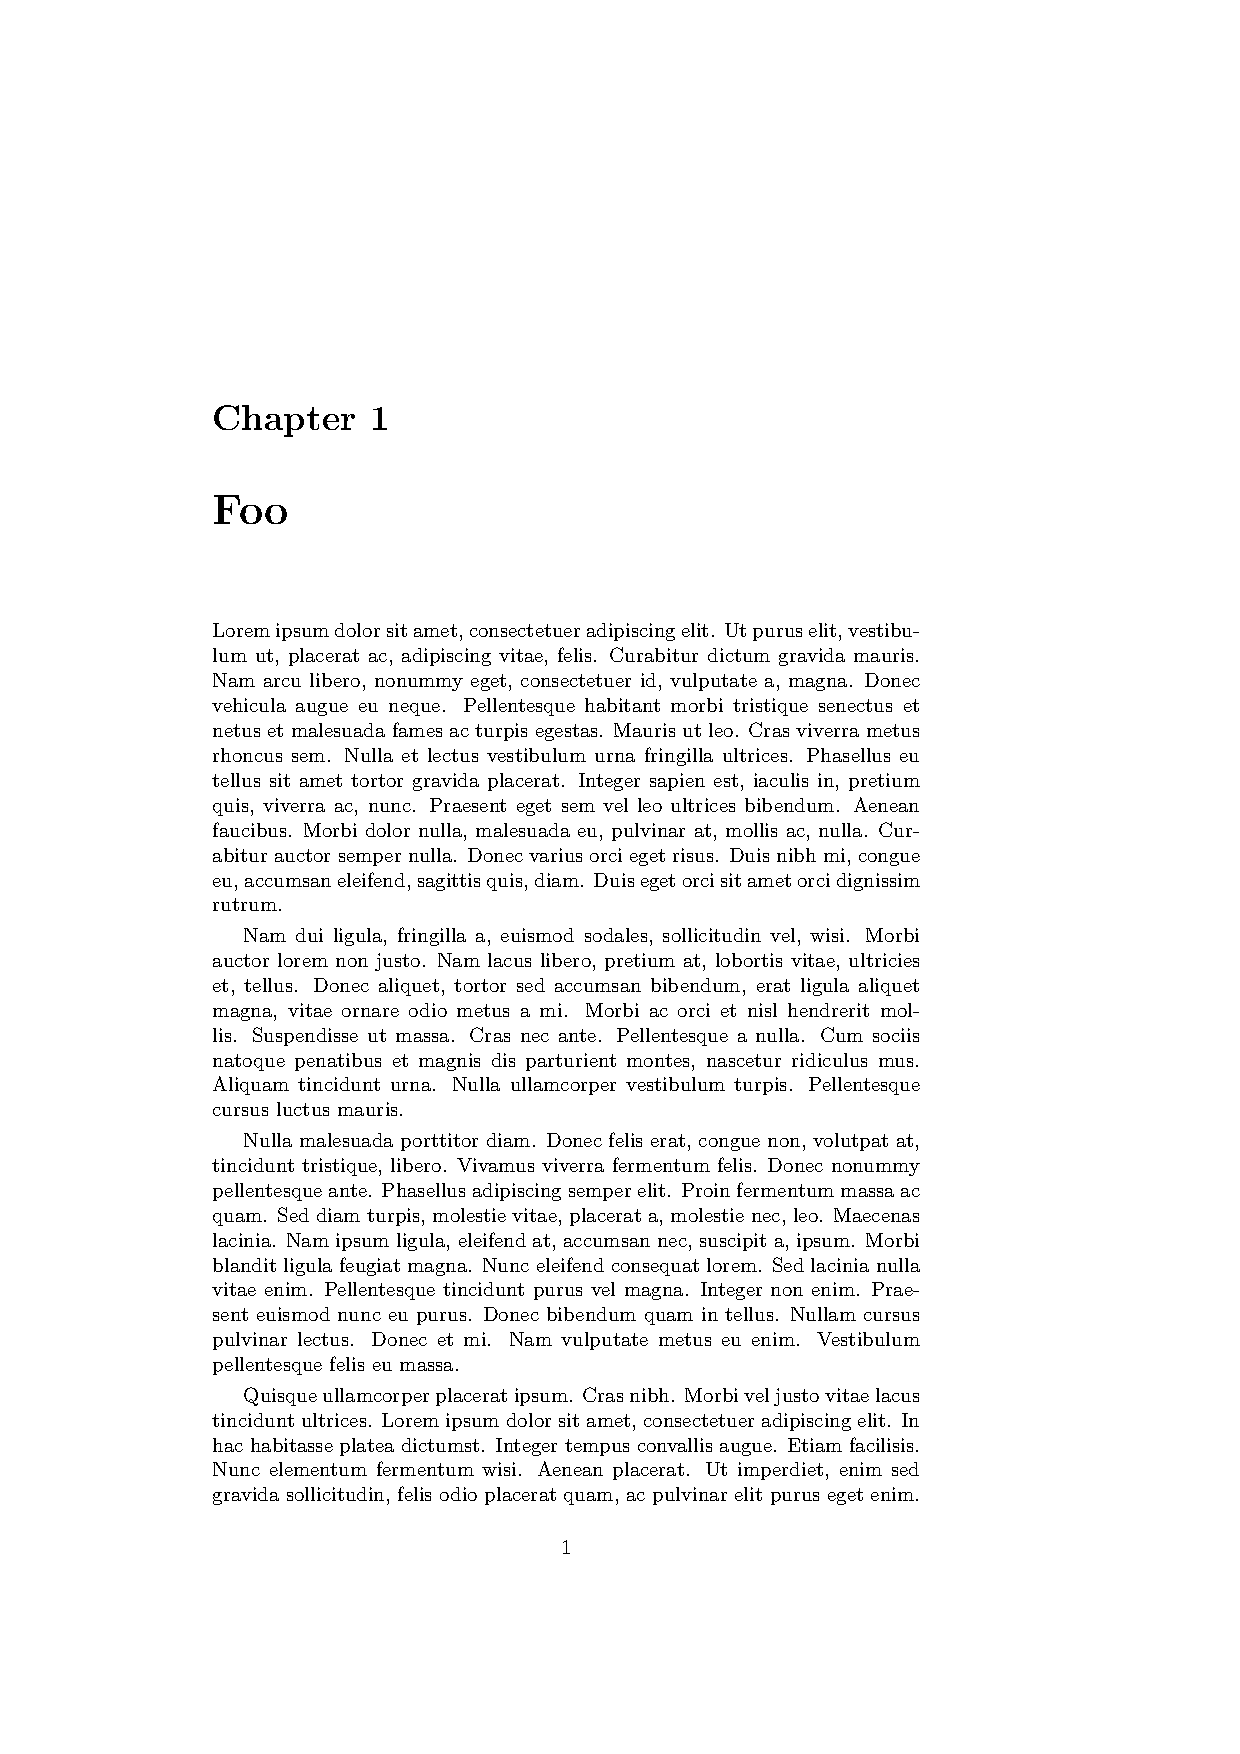
\includegraphics[frame,page=1,width=0.8\linewidth]{examples/afterchapternum}
        \end{center}
      \end{column}

      \begin{column}{0.5\textwidth}
        \begin{latexcode}
          \setlength\midchapskip{0pt}
        \end{latexcode}
        \begin{center}
          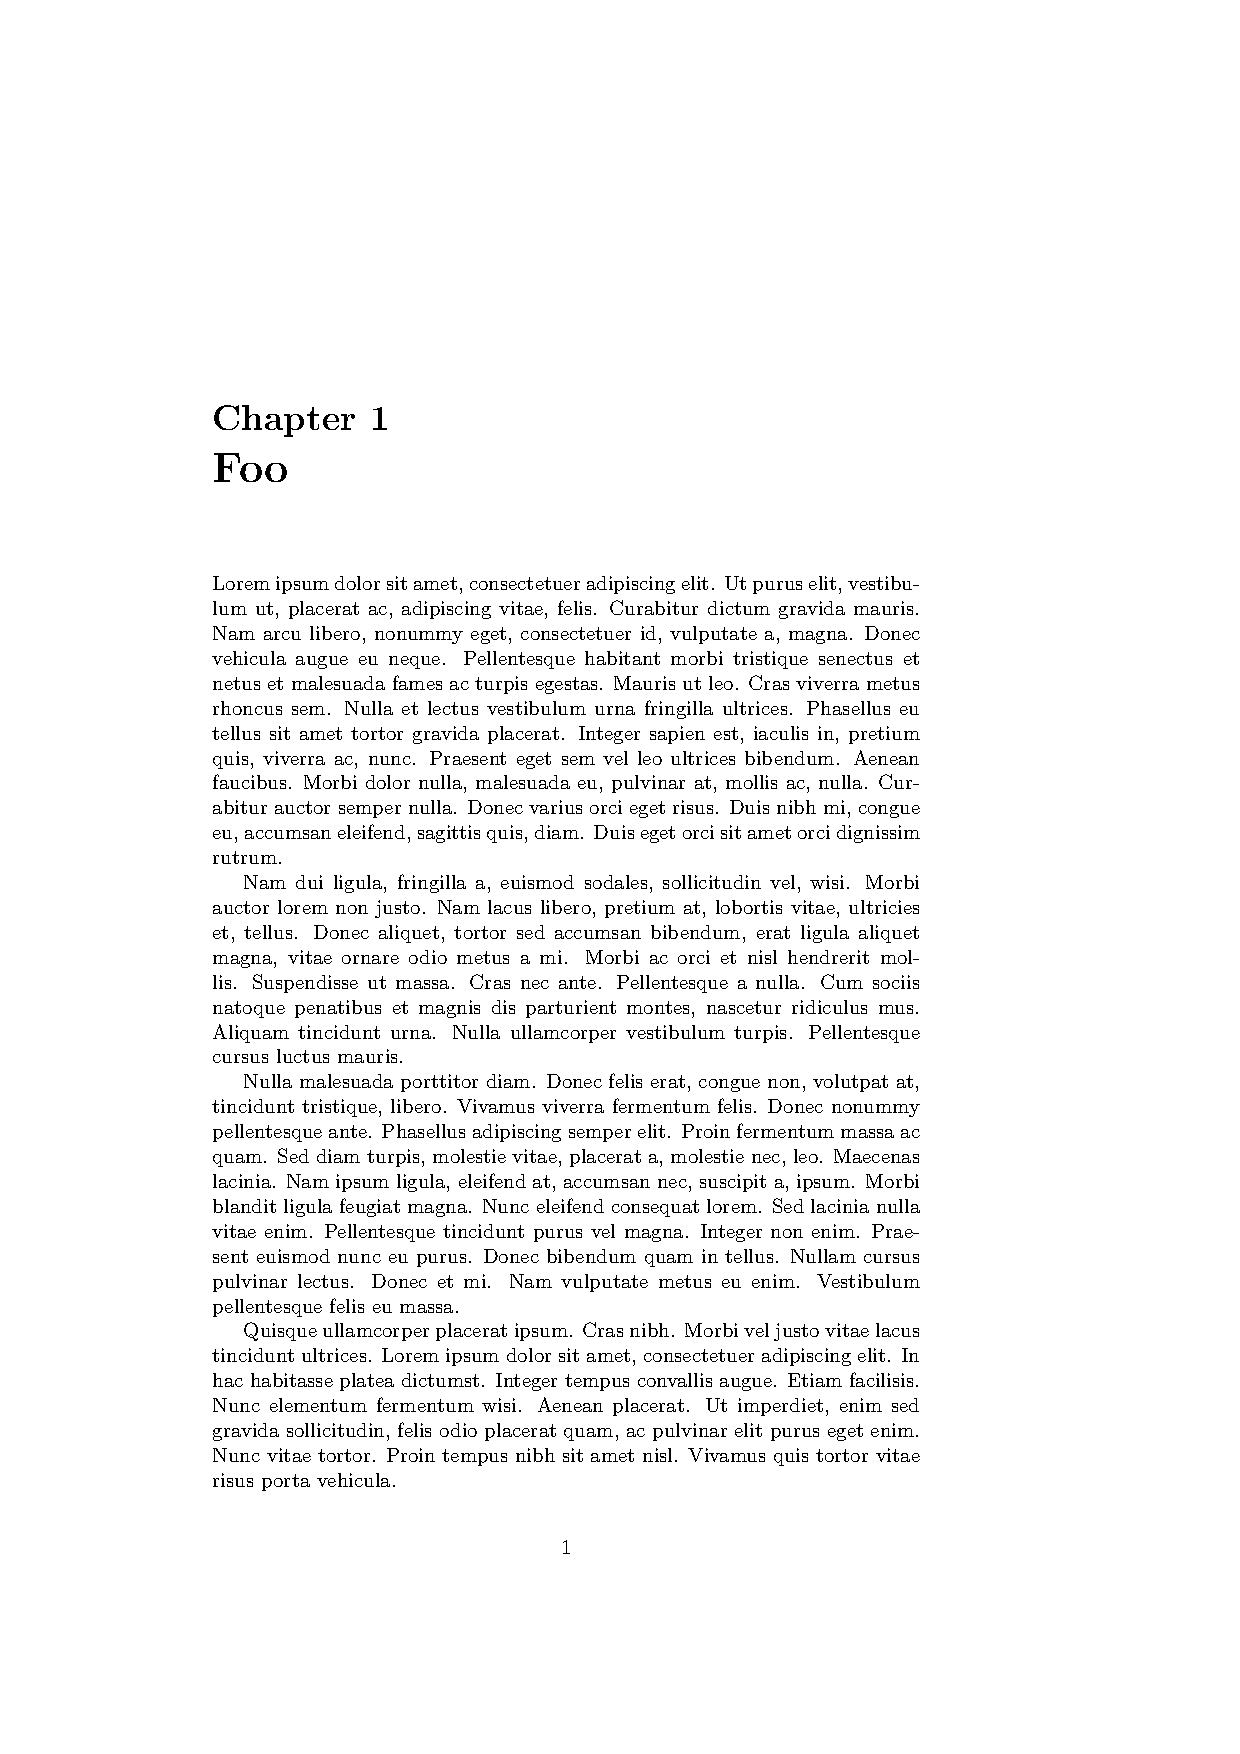
\includegraphics[frame,page=1,width=0.8\linewidth]{examples/afterchapternum-2}
        \end{center}
      \end{column}
    \end{columns}

    \onslide<2>
    \begin{columns}
      \begin{column}{0.5\textwidth}
        \begin{latexcode}
          \setlength\midchapskip{20pt}
        \end{latexcode}
        \begin{center}
          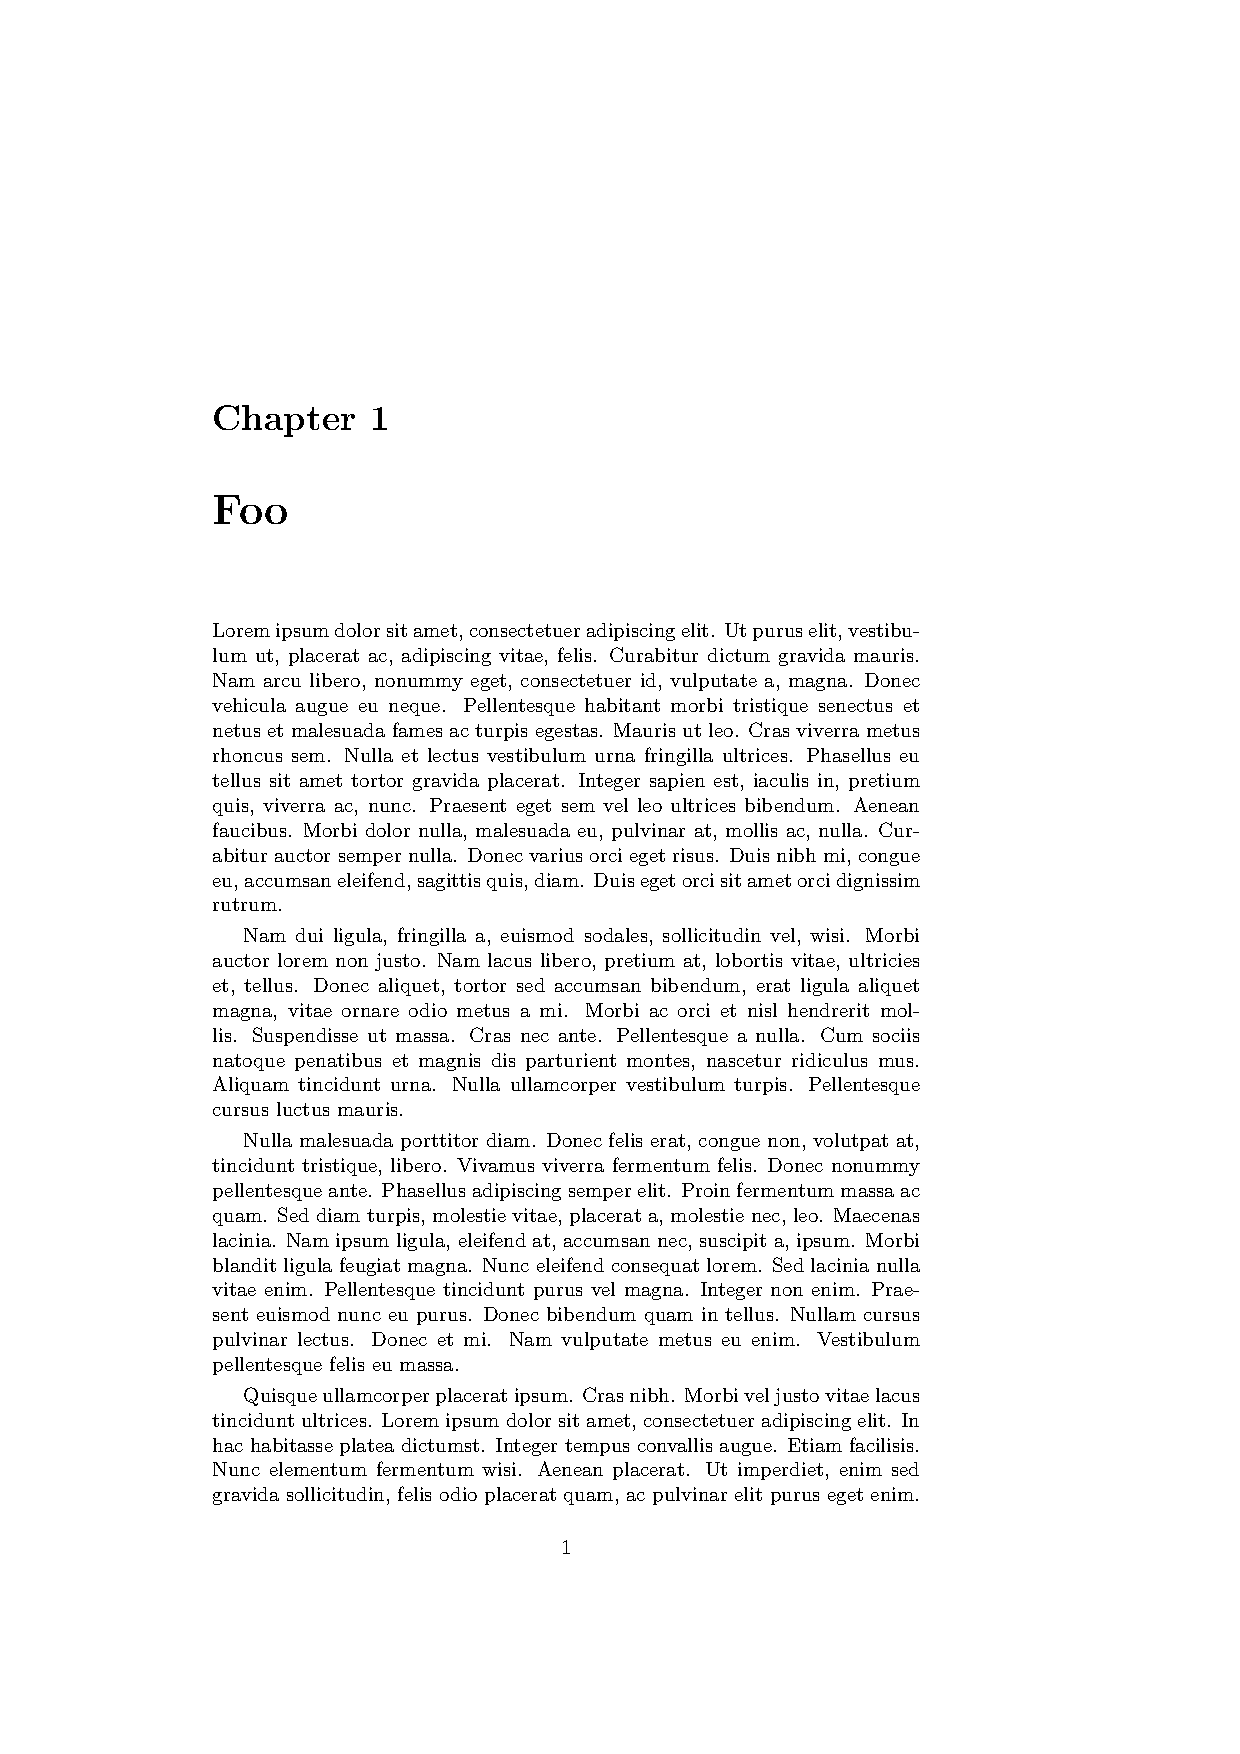
\includegraphics[frame,page=1,width=0.8\linewidth]{examples/afterchapternum}
        \end{center}
      \end{column}

      \begin{column}{0.5\textwidth}
        \begin{minted}[mathescape,
                       escapeinside=||,
                       autogobble,
                       linenos,
                       numbersep=5pt,
                       frame=single,
                       fontsize=\tiny]{latex}
          \renewcommand*{\afterchapternum}{\par\nobreak\vskip 0pt}|\vphantom{\LARGE a}|
        \end{minted}
        \begin{center}
          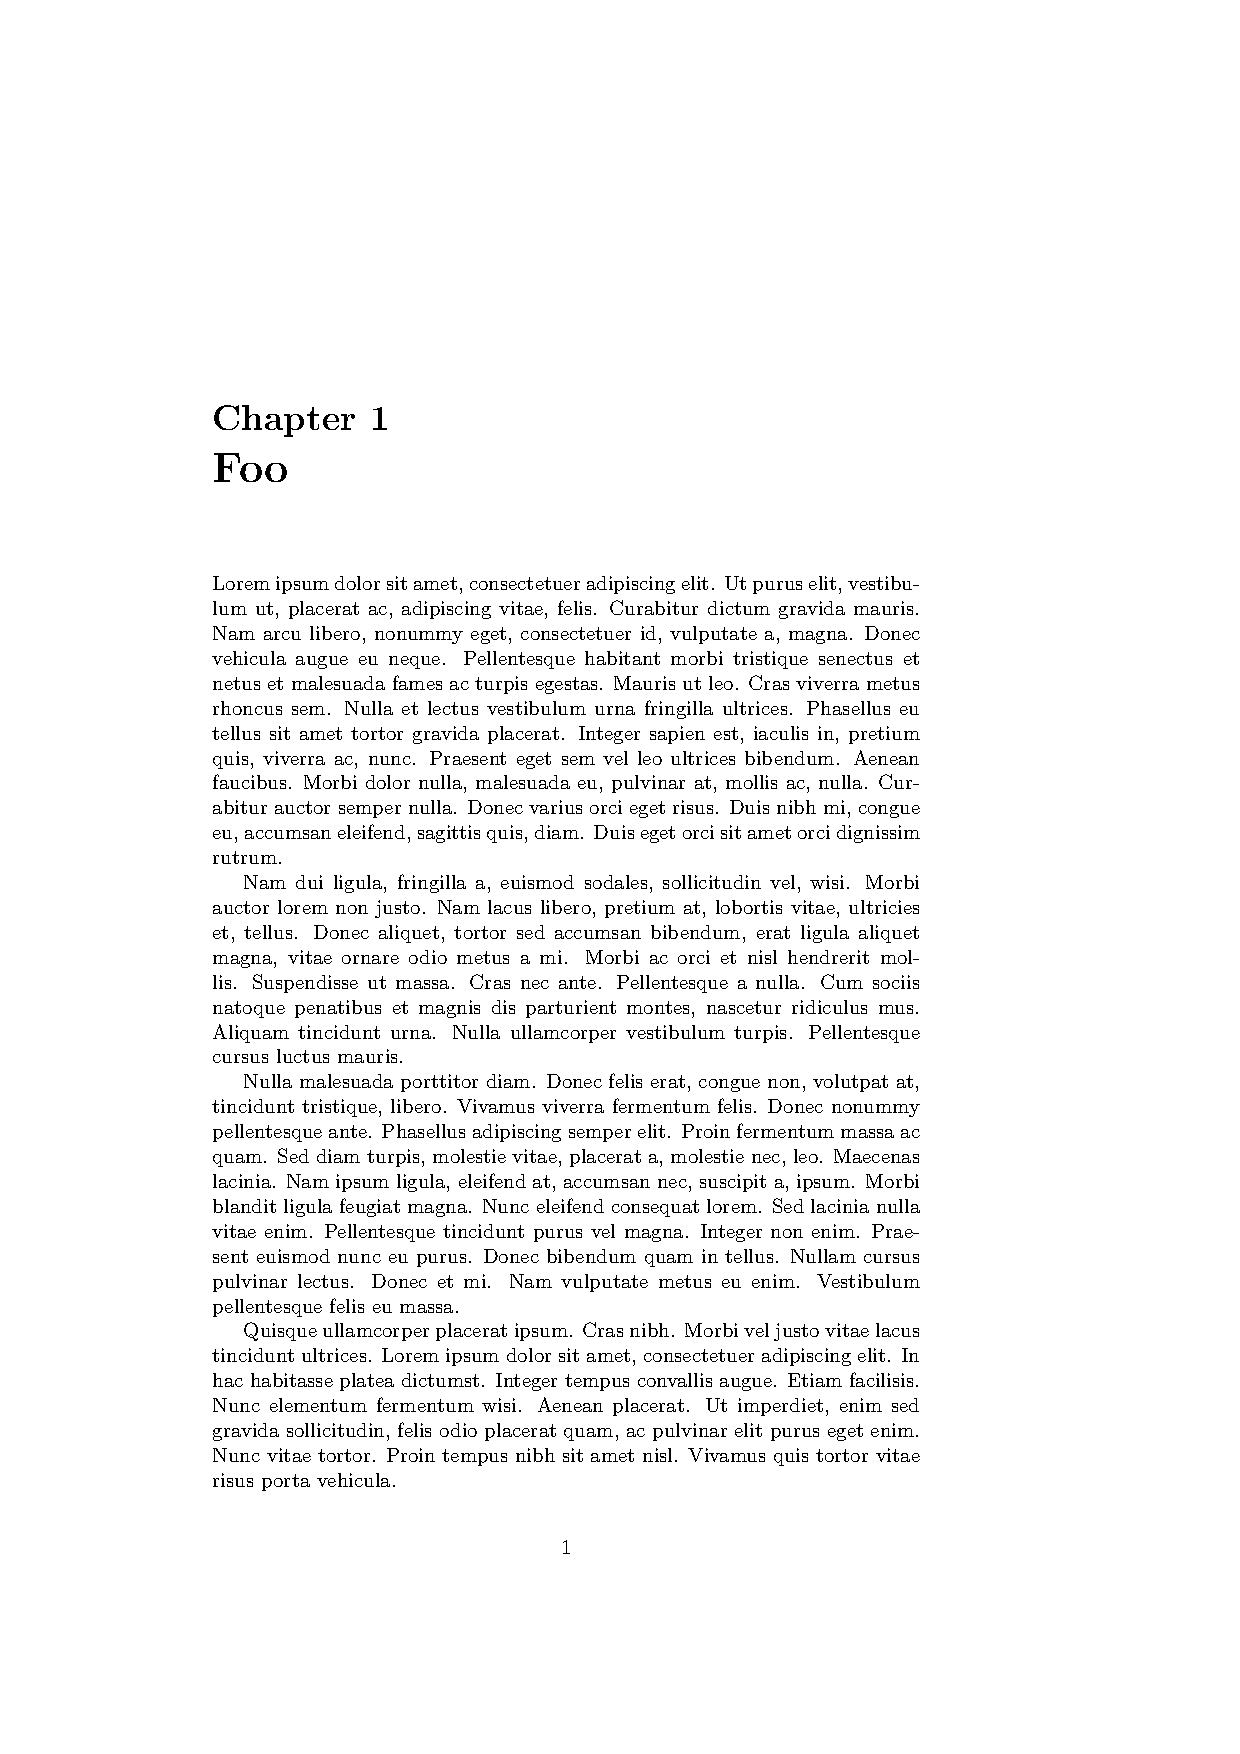
\includegraphics[frame,page=1,width=0.8\linewidth]{examples/afterchapternum-3}
        \end{center}
      \end{column}
    \end{columns}
  \end{overprint}
\end{frame}

\begin{frame}[fragile]
  {\texttt{\tbs afterchaptertitle}과 \texttt{\tbs afterchapskip} 분석}
  \ltxverb/\afterchaptertitle/은 챕터 제목을 출력한 직후에 실행되며,
  기본적으로는 40pt로 설정되어 있는 \ltxverb/\afterchapskip/을 출력한다.
\end{frame}

\begin{frame}[fragile]
  {\texttt{\tbs afterchaptertitle}과 \texttt{\tbs afterchapskip} 예시}
  \begin{overprint}
    \onslide<1>
    \begin{columns}
      \begin{column}{0.5\textwidth}
        \begin{latexcode}
          \setlength\afterchapskip{40pt}
        \end{latexcode}
        \begin{center}
          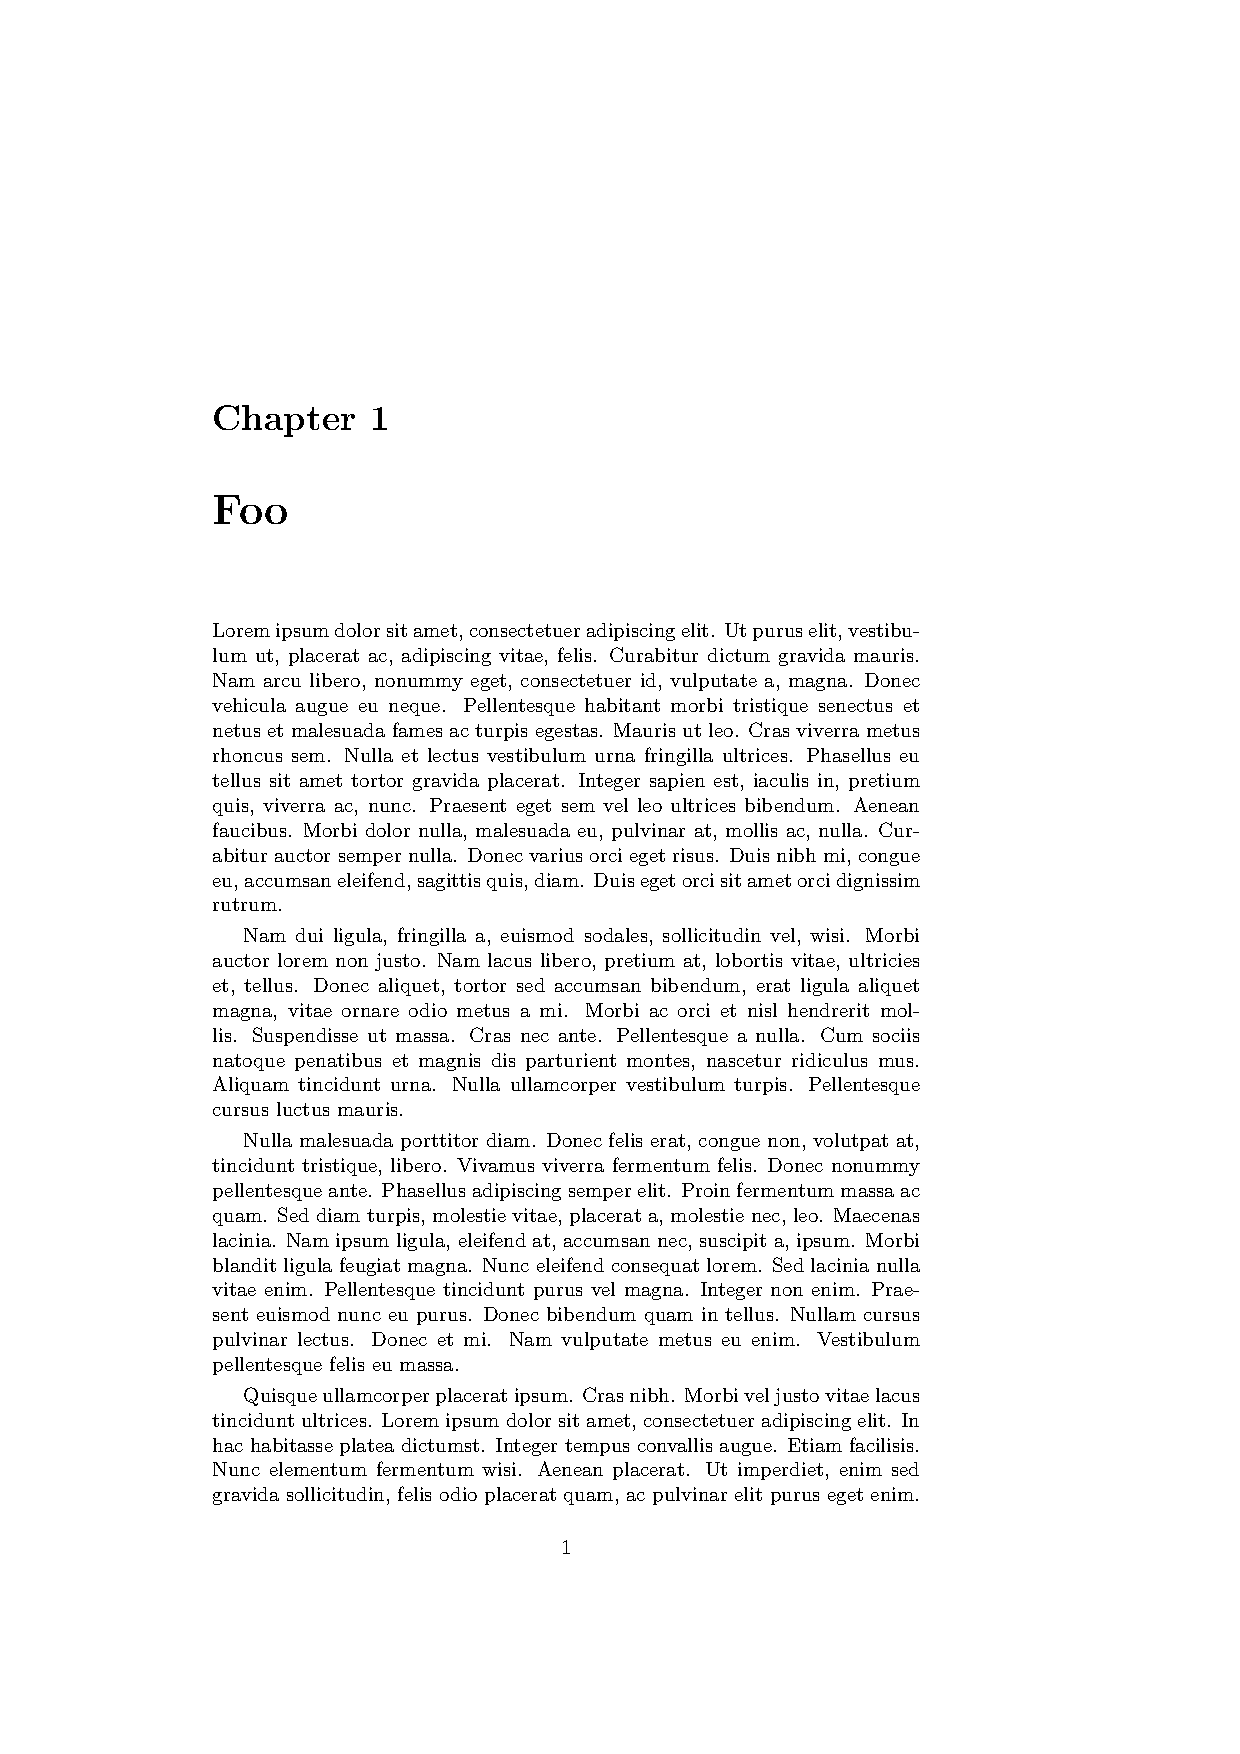
\includegraphics[frame,page=1,width=0.8\linewidth]{examples/afterchaptertitle}
        \end{center}
      \end{column}

      \begin{column}{0.5\textwidth}
        \begin{latexcode}
          \setlength\afterchapskip{0pt}
        \end{latexcode}
        \begin{center}
          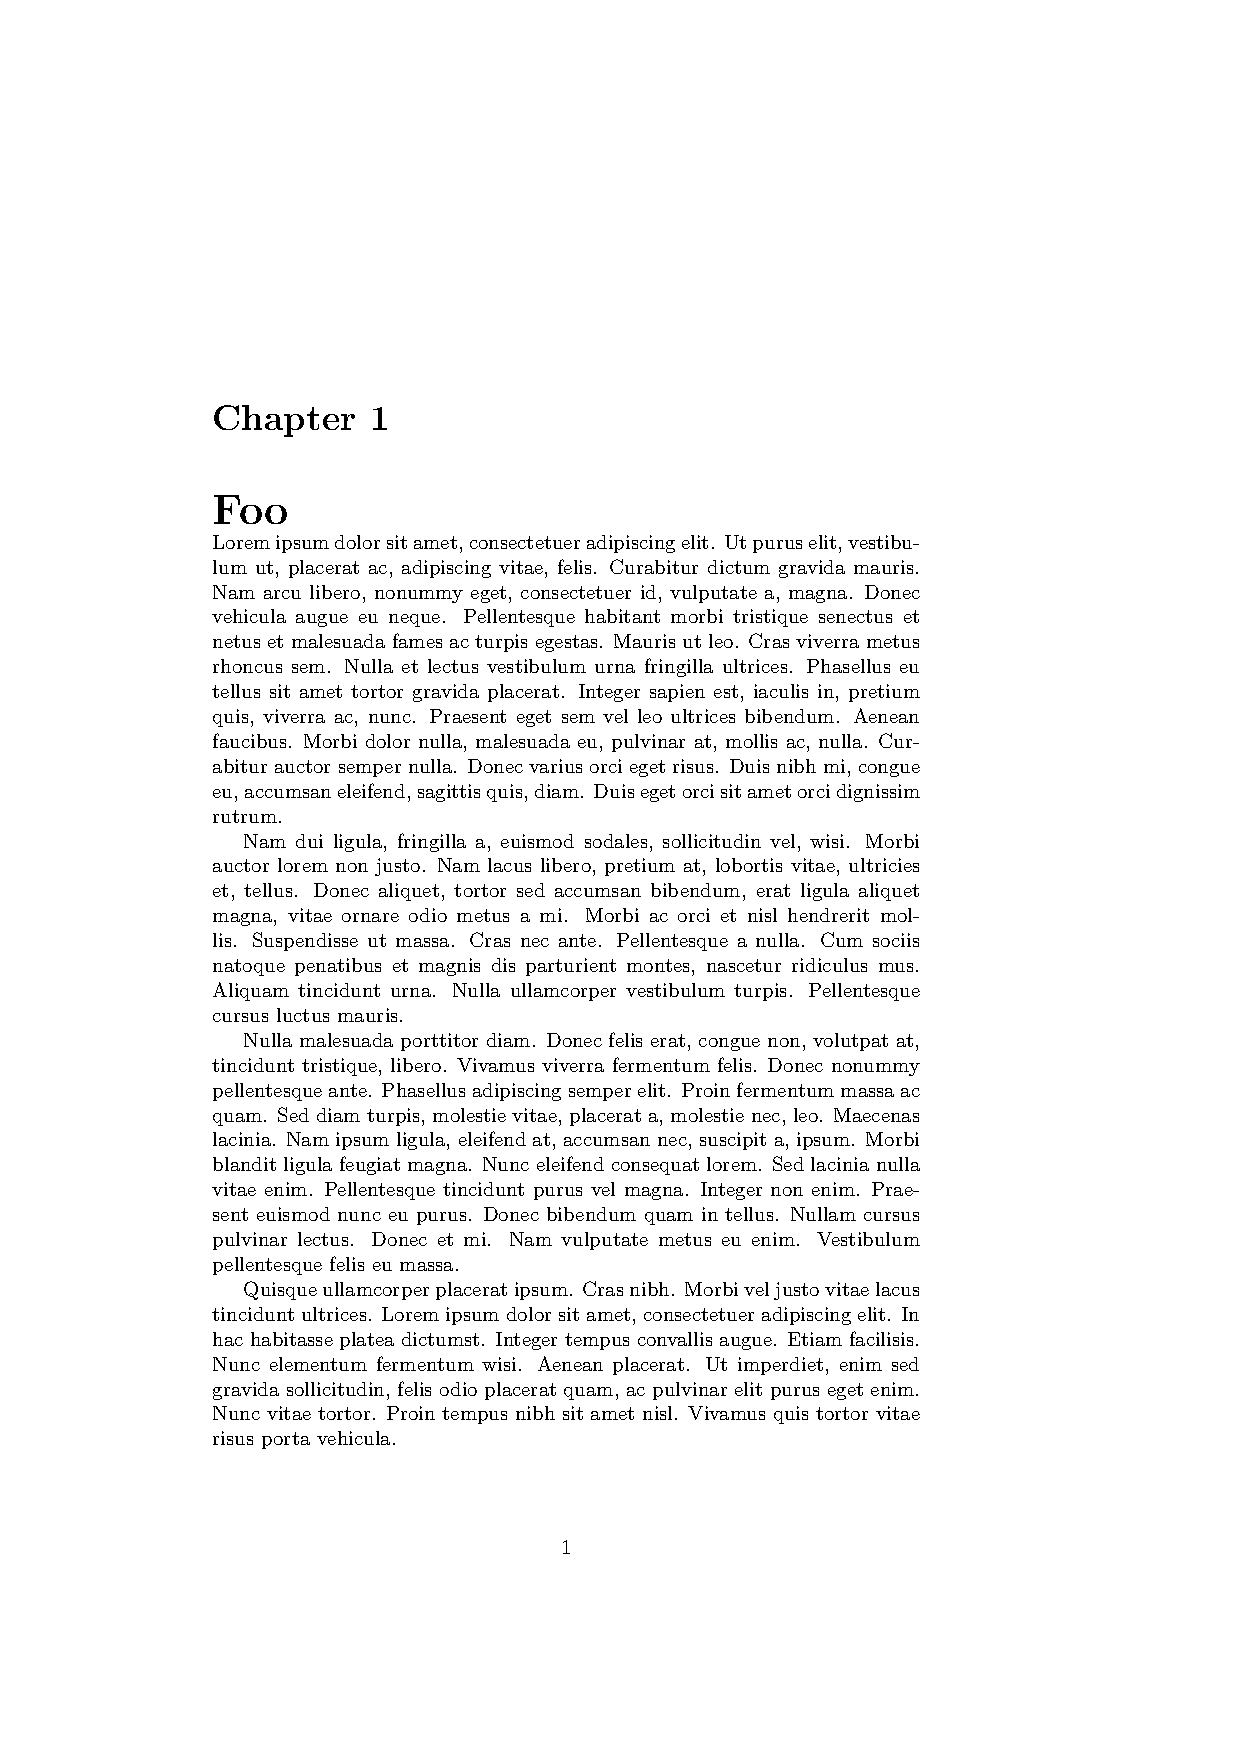
\includegraphics[frame,page=1,width=0.8\linewidth]{examples/afterchaptertitle-2}
        \end{center}
      \end{column}
    \end{columns}

    \onslide<2>
    \begin{columns}
      \begin{column}{0.5\textwidth}
        \begin{latexcode}
          \setlength\afterchapskip{40pt}
        \end{latexcode}
        \begin{center}
          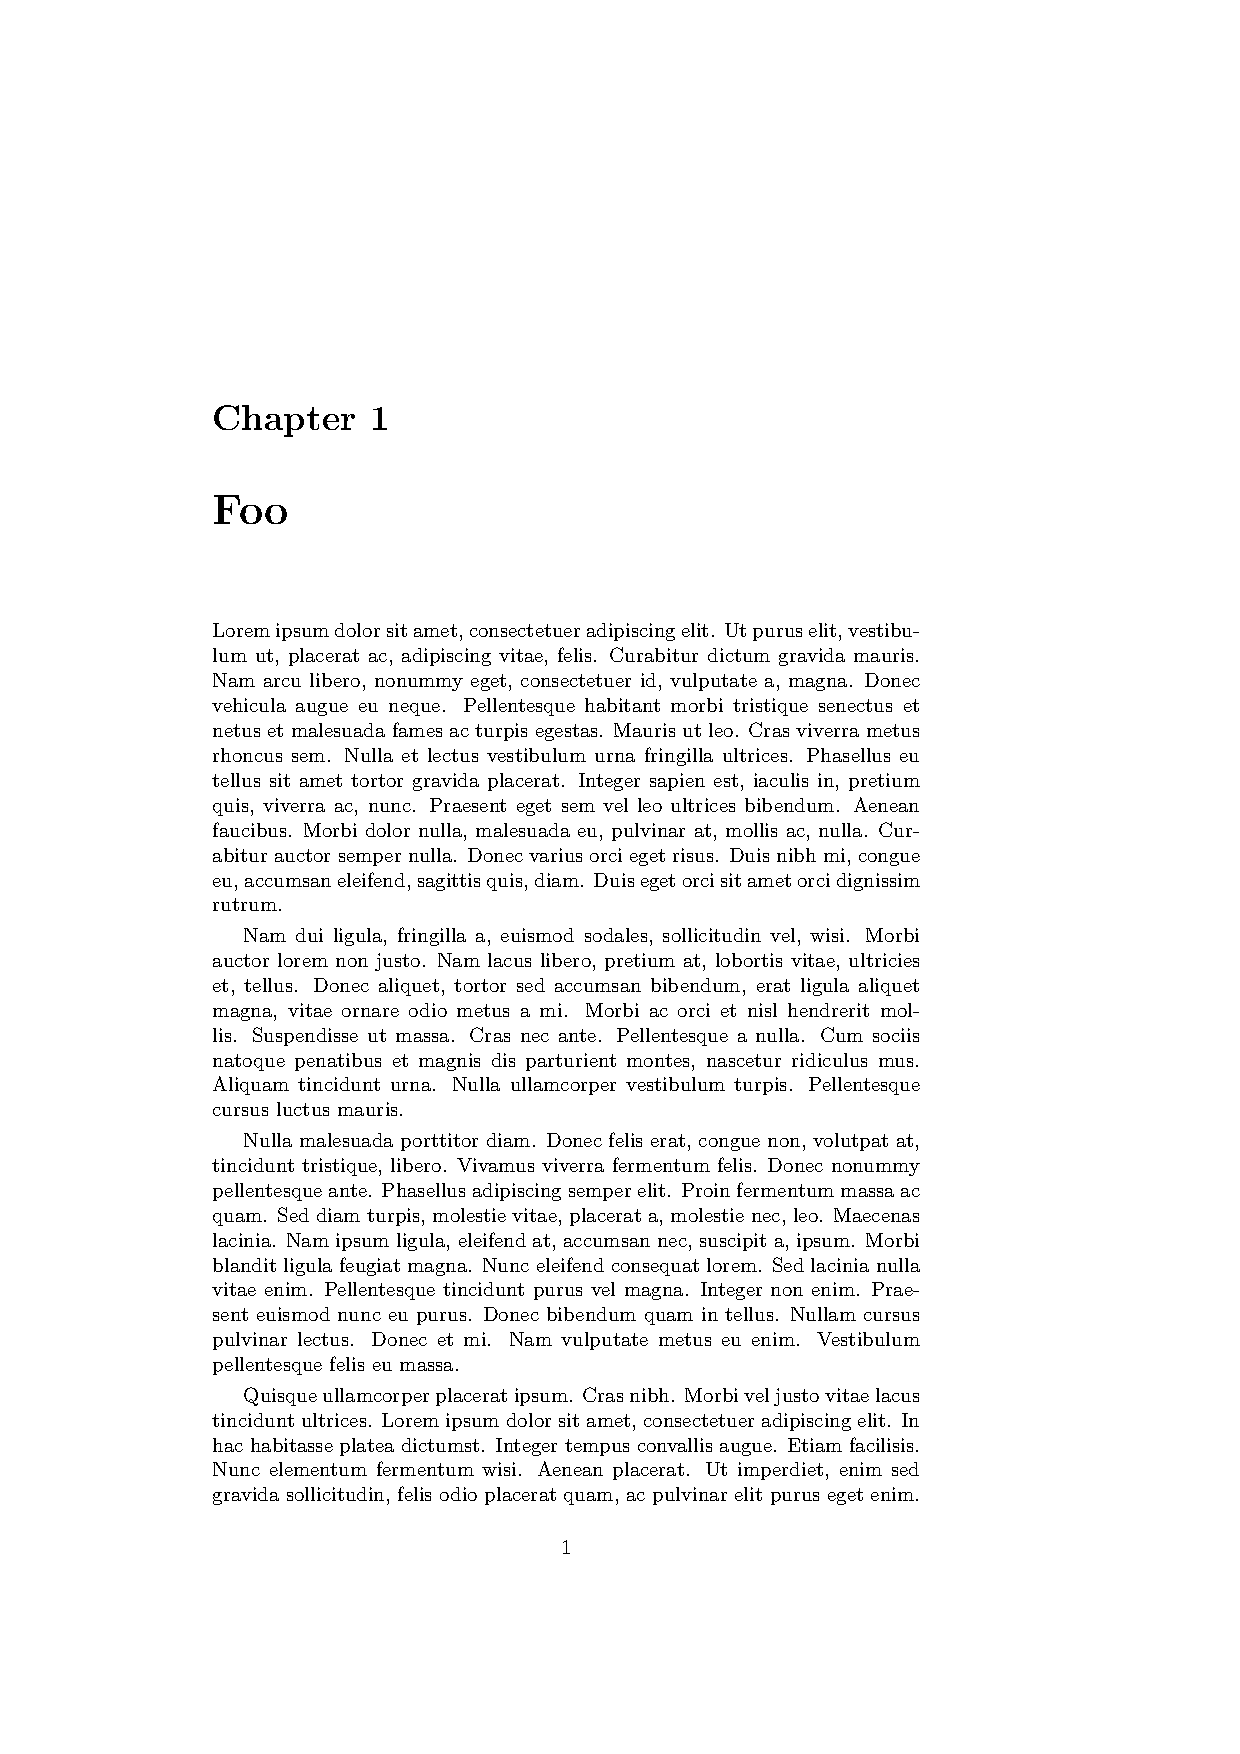
\includegraphics[frame,page=1,width=0.8\linewidth]{examples/afterchaptertitle}
        \end{center}
      \end{column}

      \begin{column}{0.5\textwidth}
        \begin{minted}[mathescape,
                       escapeinside=||,
                       autogobble,
                       linenos,
                       numbersep=5pt,
                       frame=single,
                       fontsize=\tiny]{latex}
          \renewcommand*{\afterchaptertitle}{\par\nobreak\vskip 0pt}|\vphantom{\LARGE a}|
        \end{minted}
        \begin{center}
          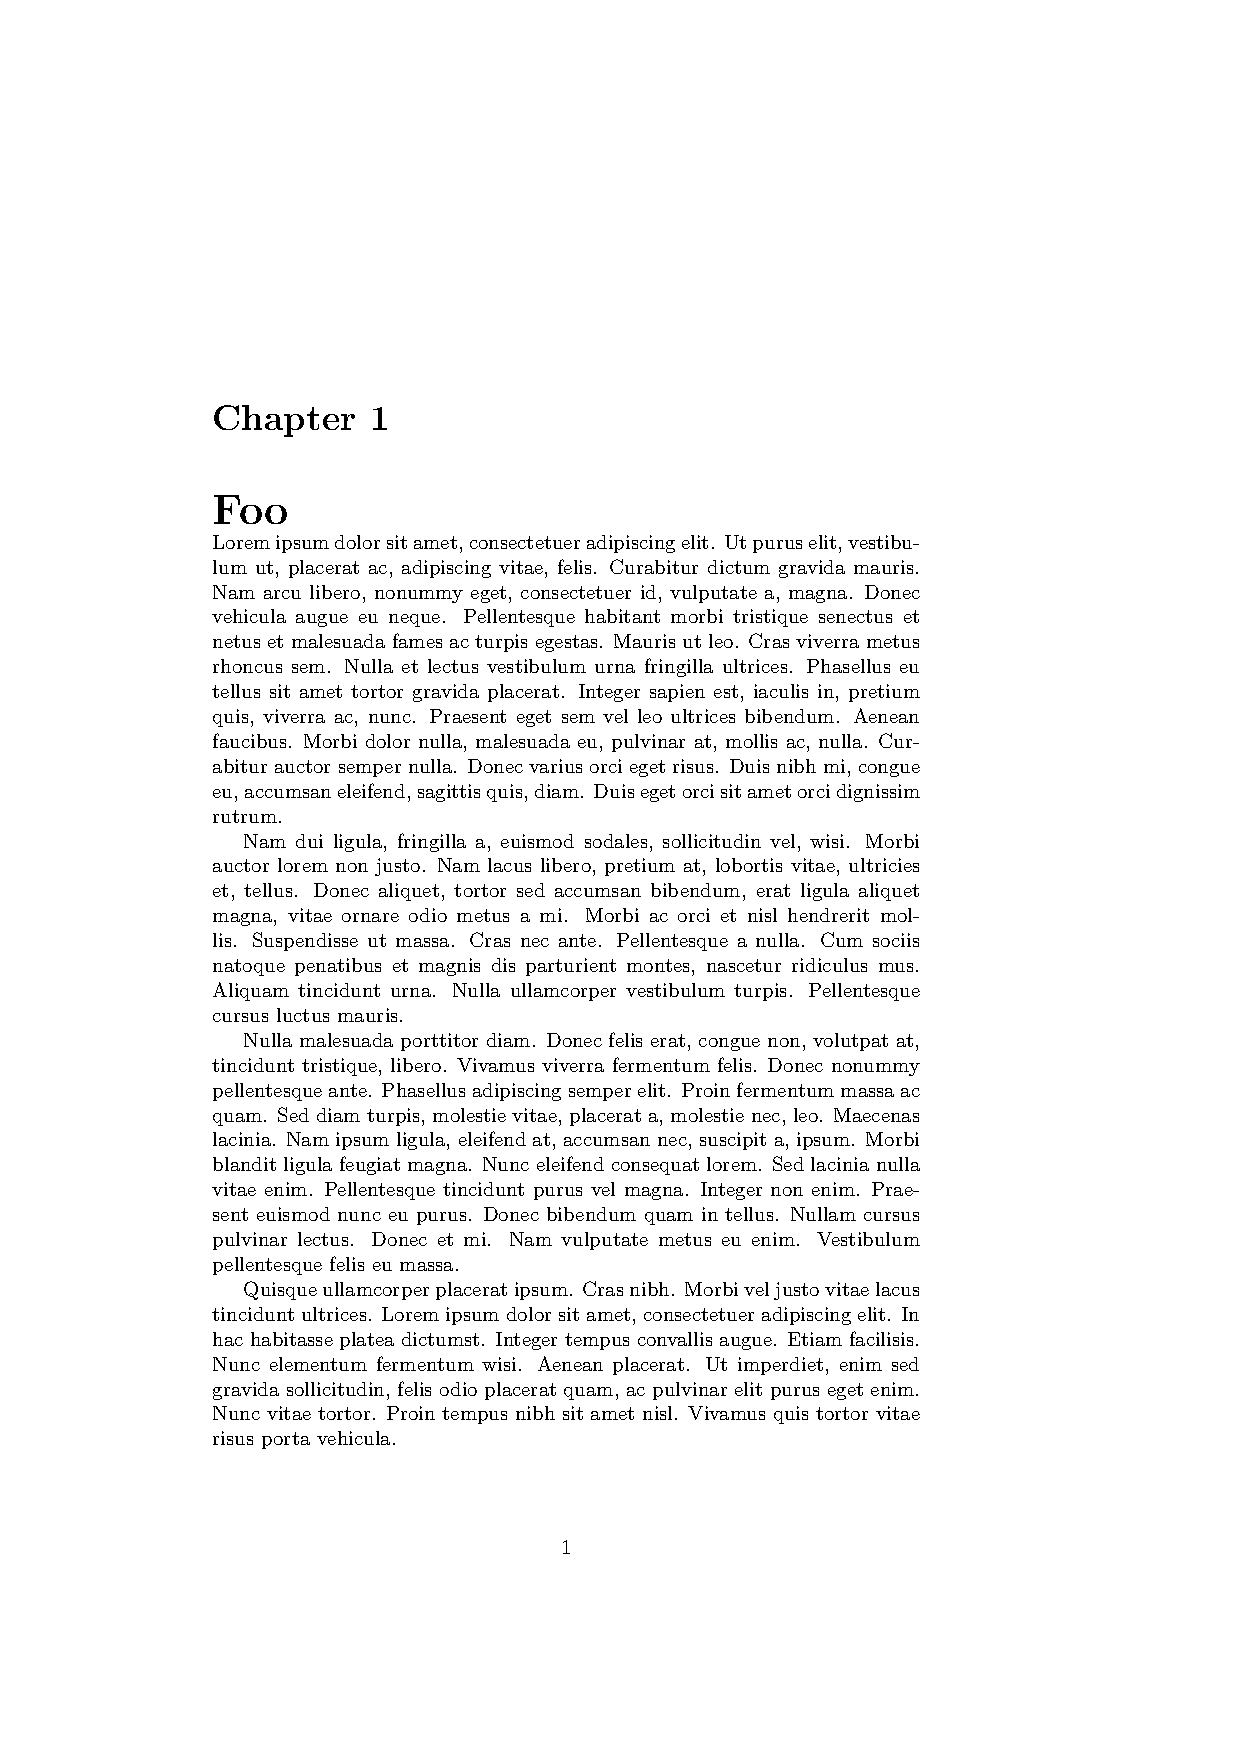
\includegraphics[frame,page=1,width=0.8\linewidth]{examples/afterchaptertitle-3}
        \end{center}
      \end{column}
    \end{columns}
  \end{overprint}
\end{frame}

\begin{frame}[fragile]
  {\texttt{\tbs printchaptername}과 \texttt{\tbs chapnamefont} 분석}
  \ltxverb/\printchaptername/은 챕터 이름을 출력한다.
  이때 이름이란 제목이 아니라, 기본적으로 \texttt{Chapter} 혹은
  \texttt{Appendix}로 정해져 있는, 챕터 앞에 붙는 이름을 말한다.
  사용되는 글꼴은 \ltxverb/\chapnamefont/로 지정하고, 기본값은
  \ltxverb/\bfseries\huge/이다.
\end{frame}

\begin{frame}[fragile]{\texttt{\tbs printchaptername} 및 \texttt{\tbs chapnamefont} 예시}
  \begin{overprint}
    \onslide<1>
    \begin{columns}
      \begin{column}{0.6\textwidth}
        \begin{latexcode}
          \renewcommand*{\printchaptername}{%
            \sffamily\large LECTURE }
        \end{latexcode}
      \end{column}

      \begin{column}{0.4\textwidth}
        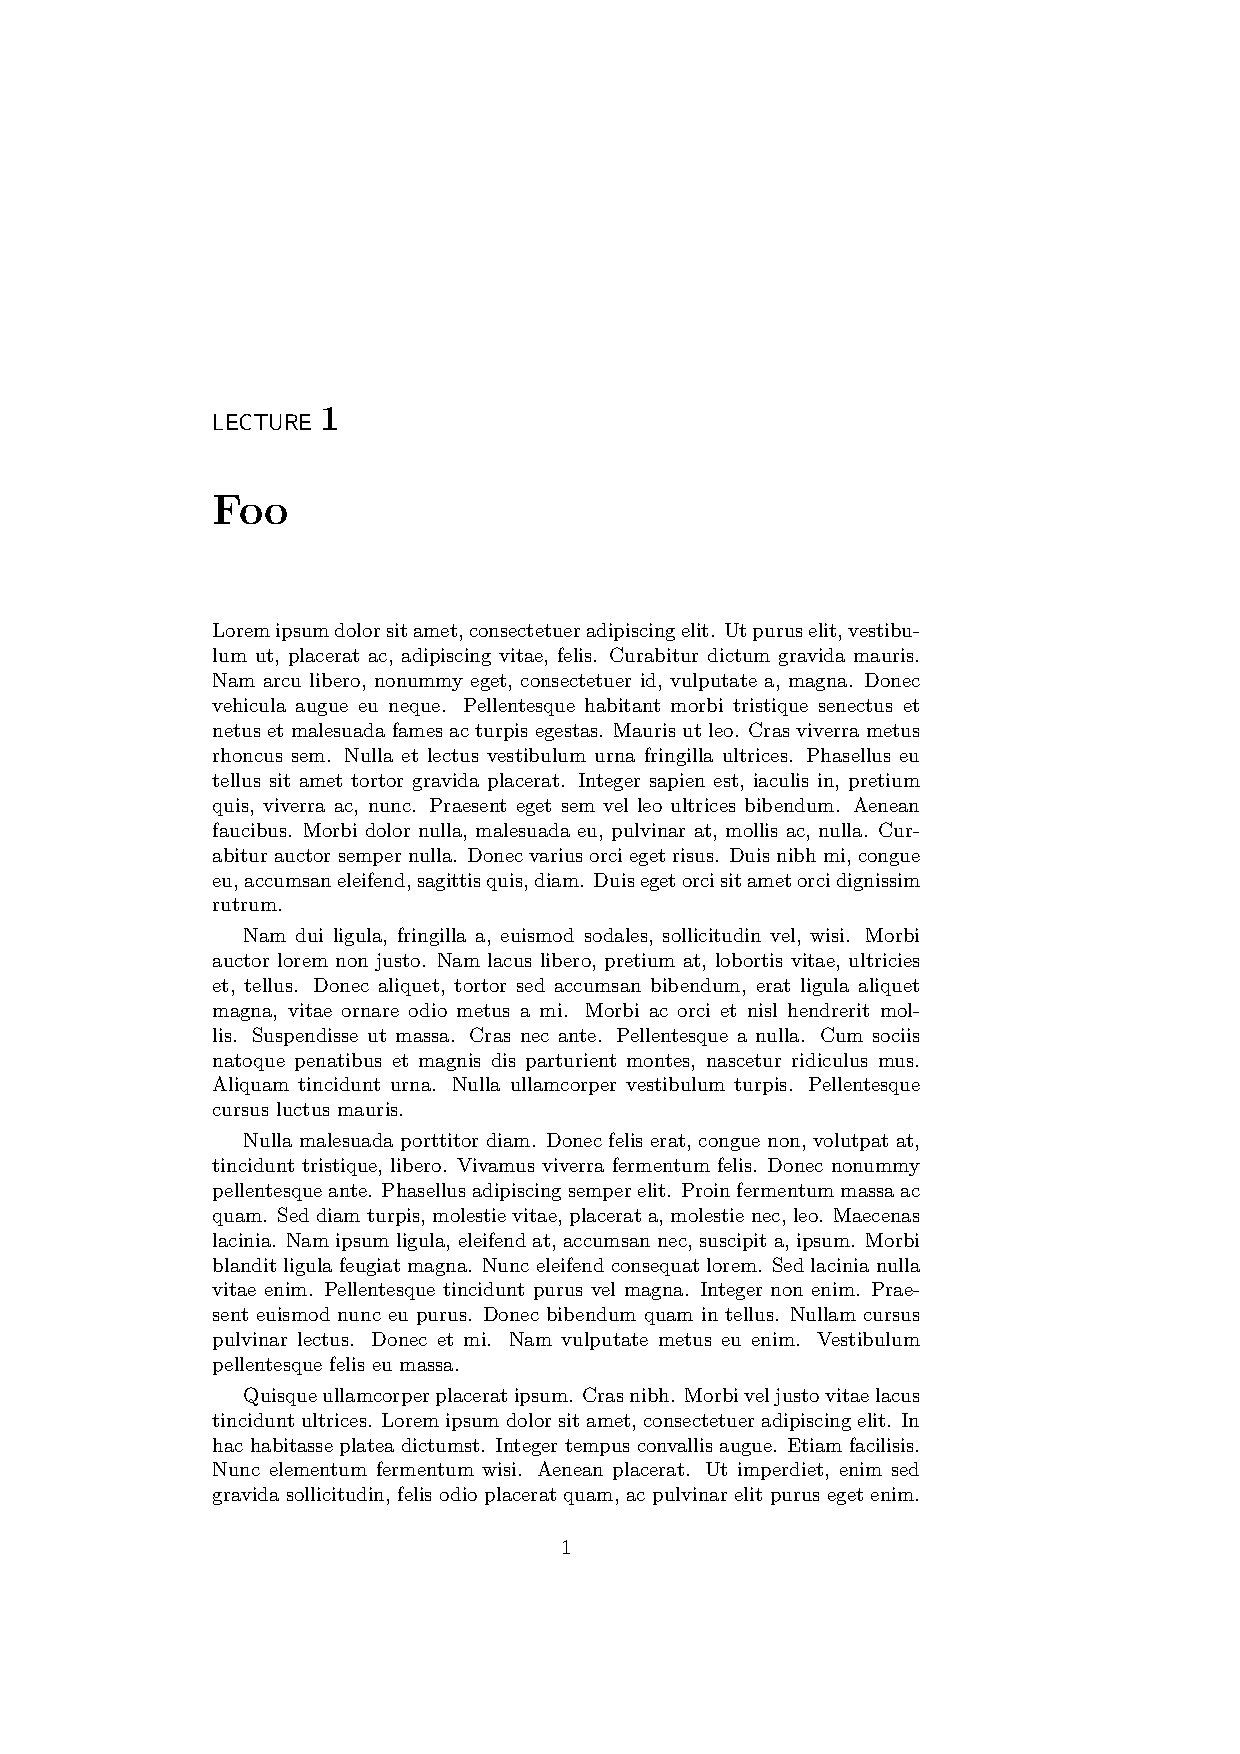
\includegraphics[frame,page=1,width=\linewidth]{examples/printchaptername}
      \end{column}
    \end{columns}

    \onslide<2>
    \begin{columns}
      \begin{column}{0.6\textwidth}
        \begin{latexcode}
          \renewcommand*{\printchaptername}{%
            \chapnamefont LECTURE }
          \renewcommand*{\chapnamefont}{\sffamily\large}
        \end{latexcode}
      \end{column}

      \begin{column}{0.4\textwidth}
        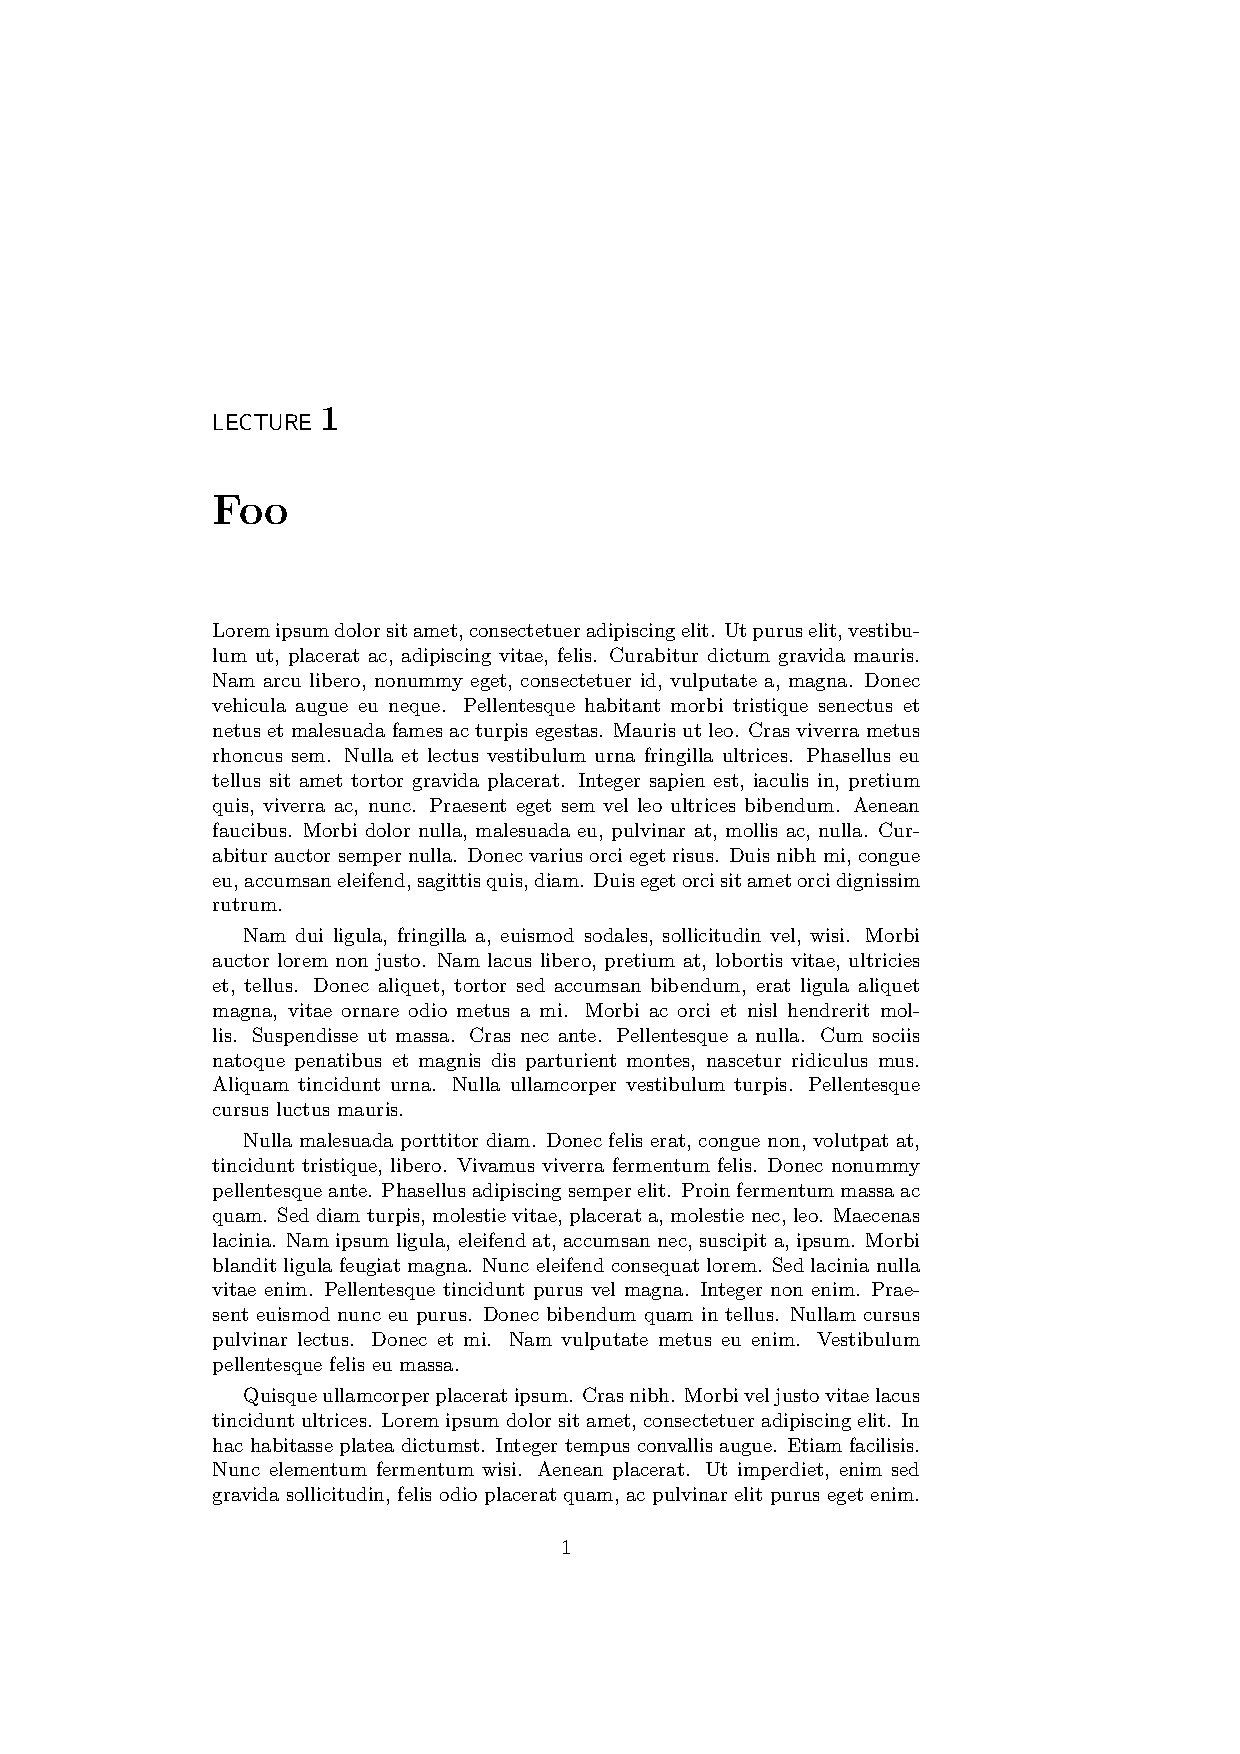
\includegraphics[frame,page=1,width=\linewidth]{examples/printchaptername}
      \end{column}
    \end{columns}

    \onslide<3>
    \begin{columns}
      \begin{column}{0.6\textwidth}
        \begin{latexcode}
          \makeatletter
          \renewcommand*{\@chapapp}{LECTURE}
          \renewcommand*{\printchaptername}{%
            \chapnamefont\@chapapp}
          \renewcommand*{\chapnamefont}{\sffamily\large}
          \makeatother
        \end{latexcode}
      \end{column}

      \begin{column}{0.4\textwidth}
        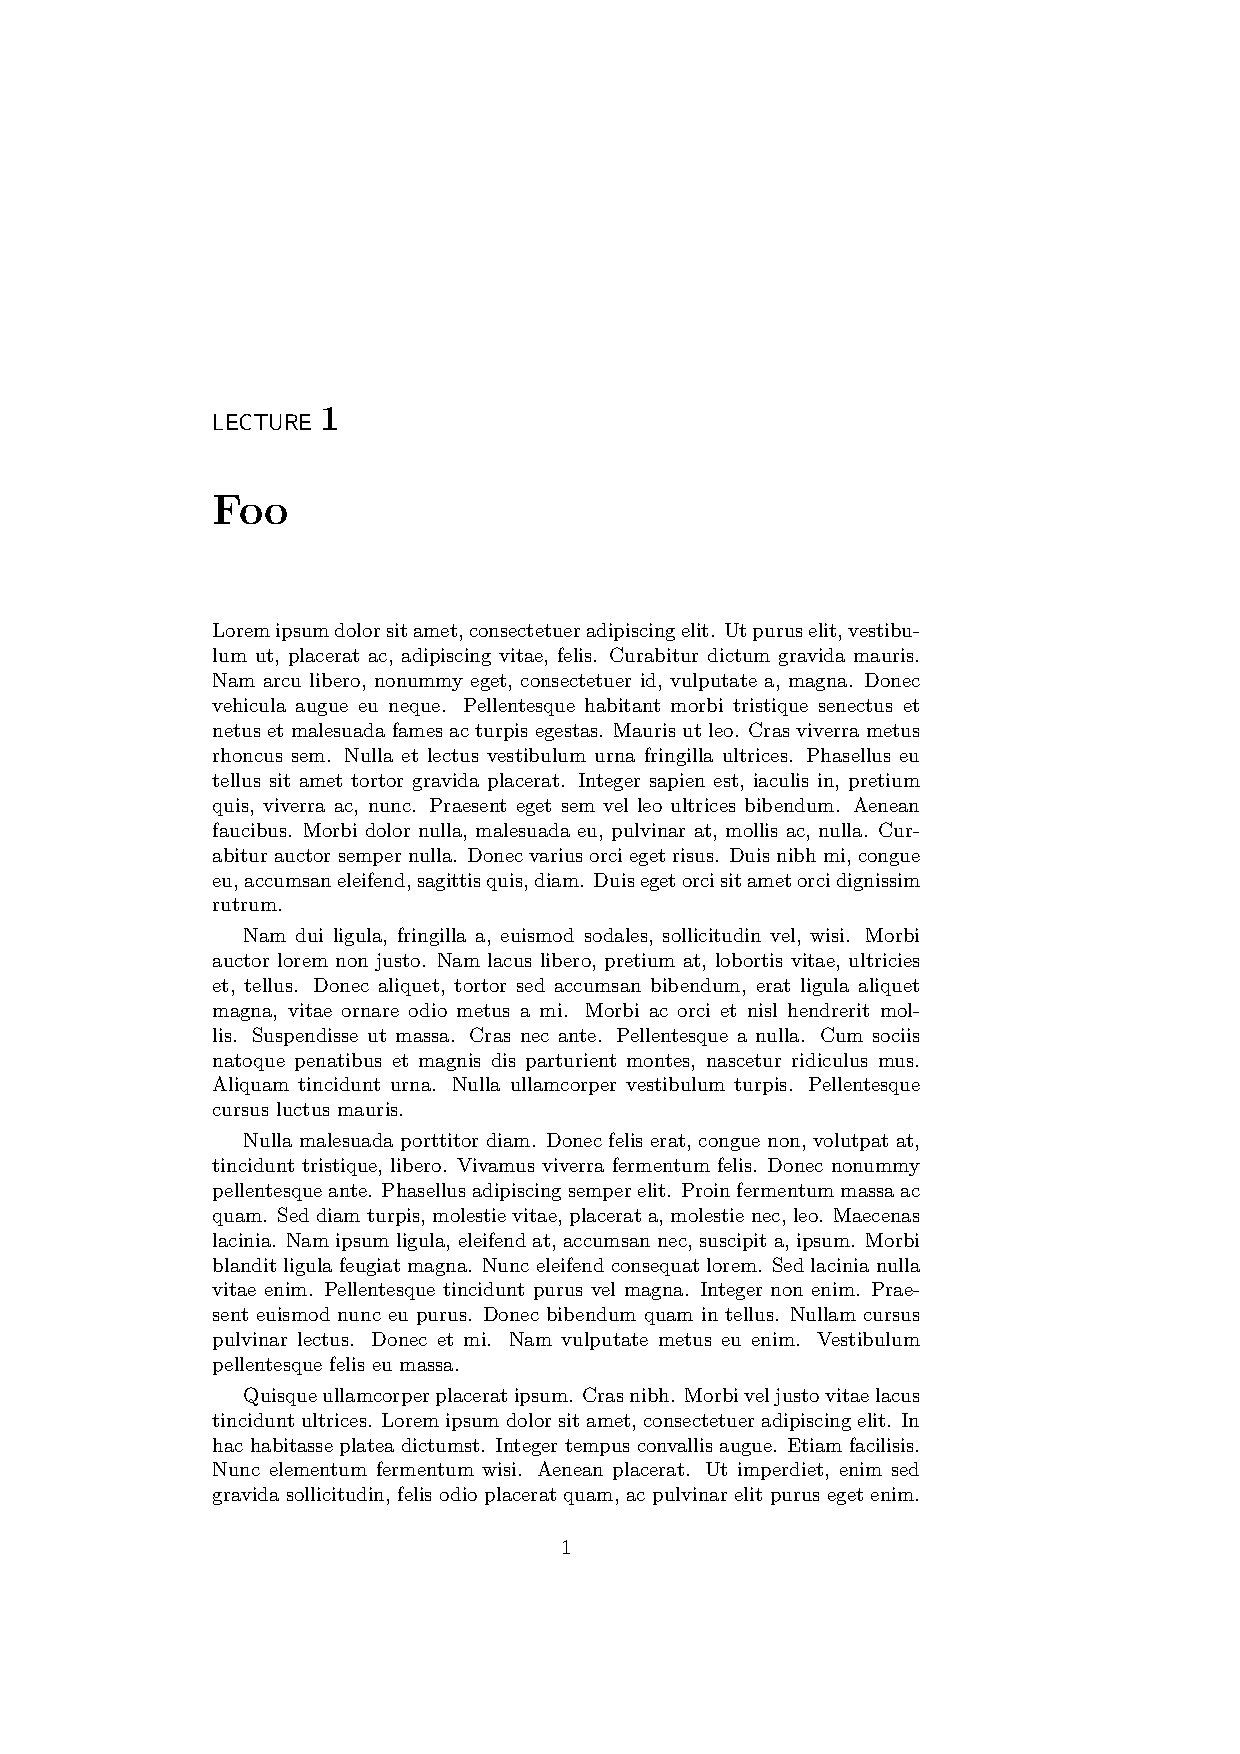
\includegraphics[frame,page=1,width=\linewidth]{examples/printchaptername}
      \end{column}
    \end{columns}

    \onslide<4>
    \begin{columns}
      \begin{column}{0.6\textwidth}
        \begin{latexcode}
          \makeatletter
          \renewcommand*{\@chapapp}{Lecture}
          \renewcommand*{\printchaptername}{%
            \chapnamefont\MakeUppercase\@chapapp}
          \renewcommand*{\chapnamefont}{\sffamily\large}
          \makeatother
        \end{latexcode}
      \end{column}

      \begin{column}{0.4\textwidth}
        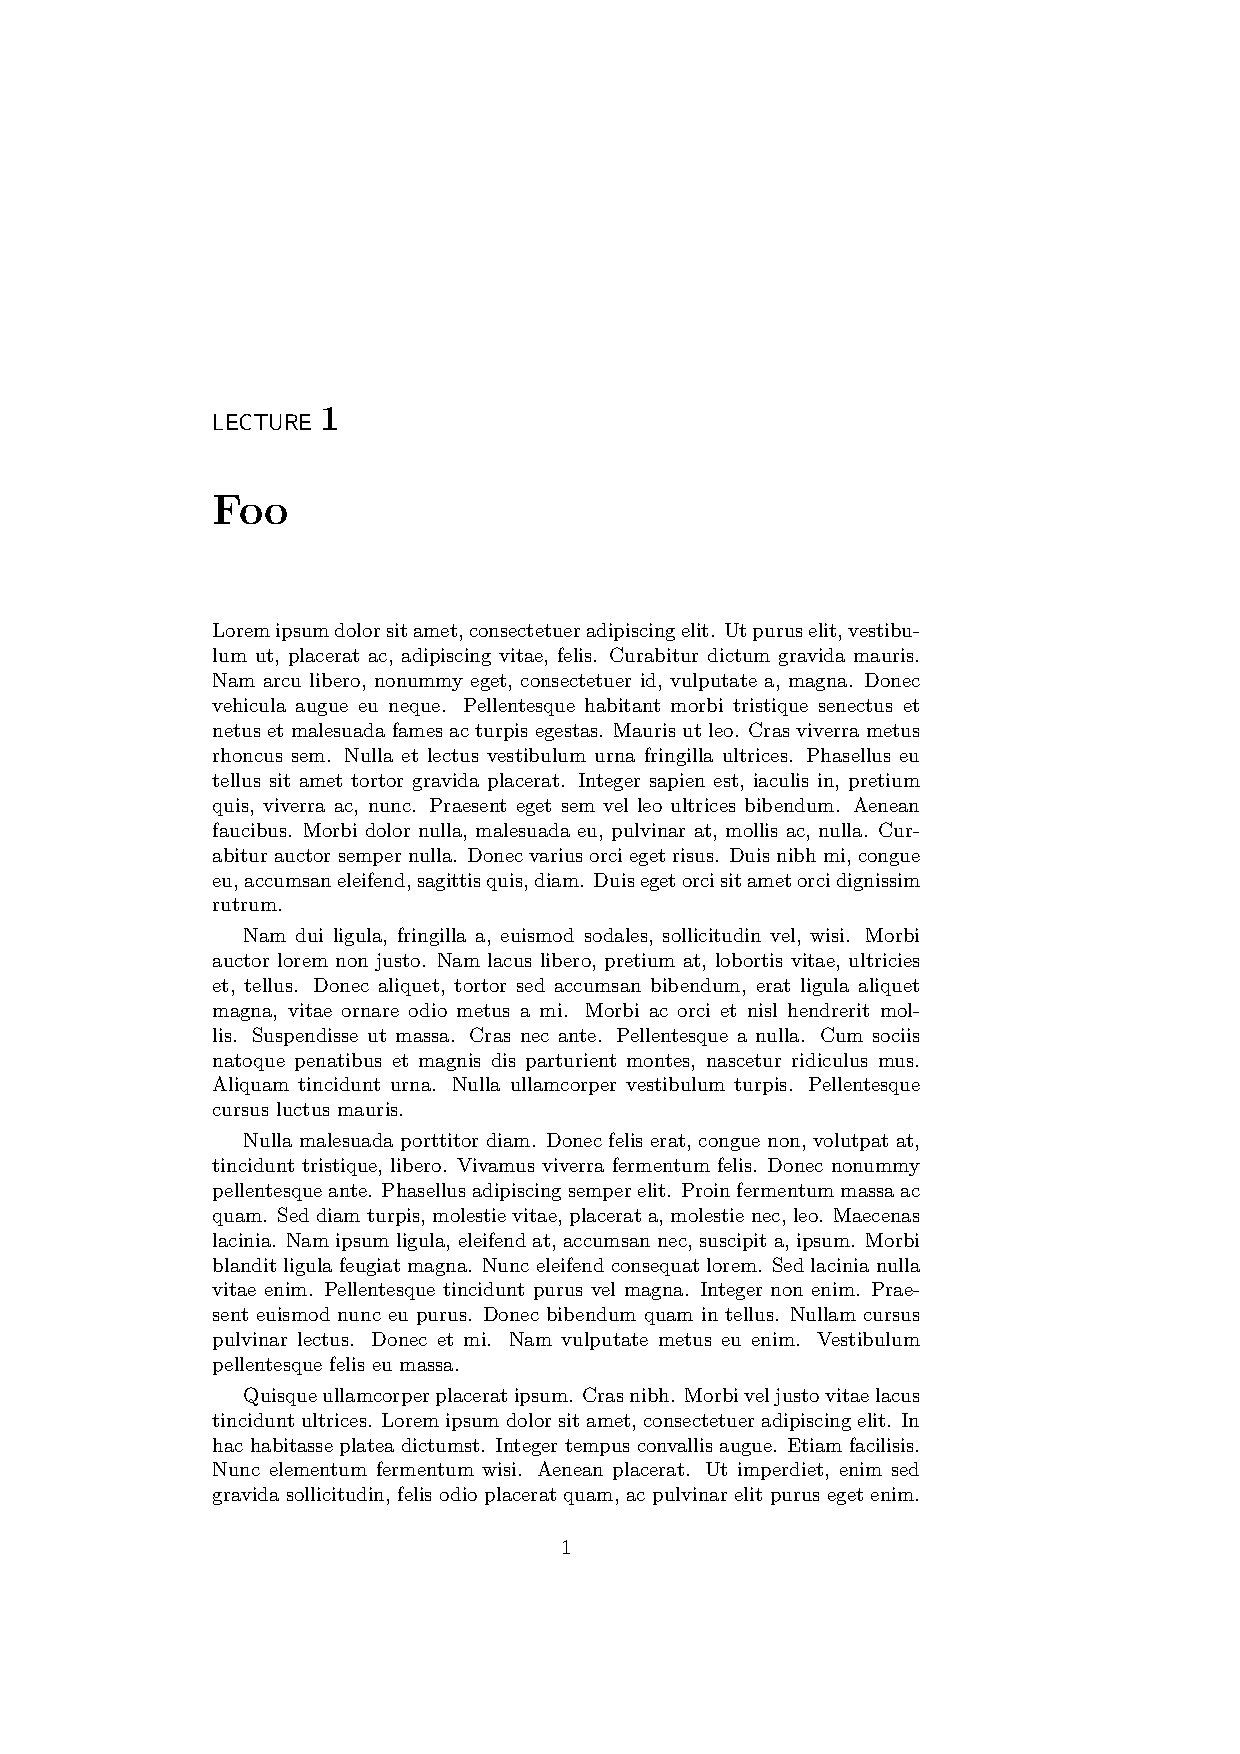
\includegraphics[frame,page=1,width=\linewidth]{examples/printchaptername}
      \end{column}
    \end{columns}
  \end{overprint}
\end{frame}

\begin{frame}[fragile]
  {\texttt{\tbs chapternamenum} 분석 및 예시}
  \begin{columns}
    \begin{column}{0.6\textwidth}
      \ltxverb/\chapternamenum/은 챕터 이름과 번호 사이에 사용되는 명령어로,
      기본값은 띄어쓰기이다.
      \pause
      \newline
      \begin{latexcode}
        \renewcommand*{\chapternamenum}{\vskip 12pt}
      \end{latexcode}
    \end{column}

    \begin{column}{0.4\textwidth}
      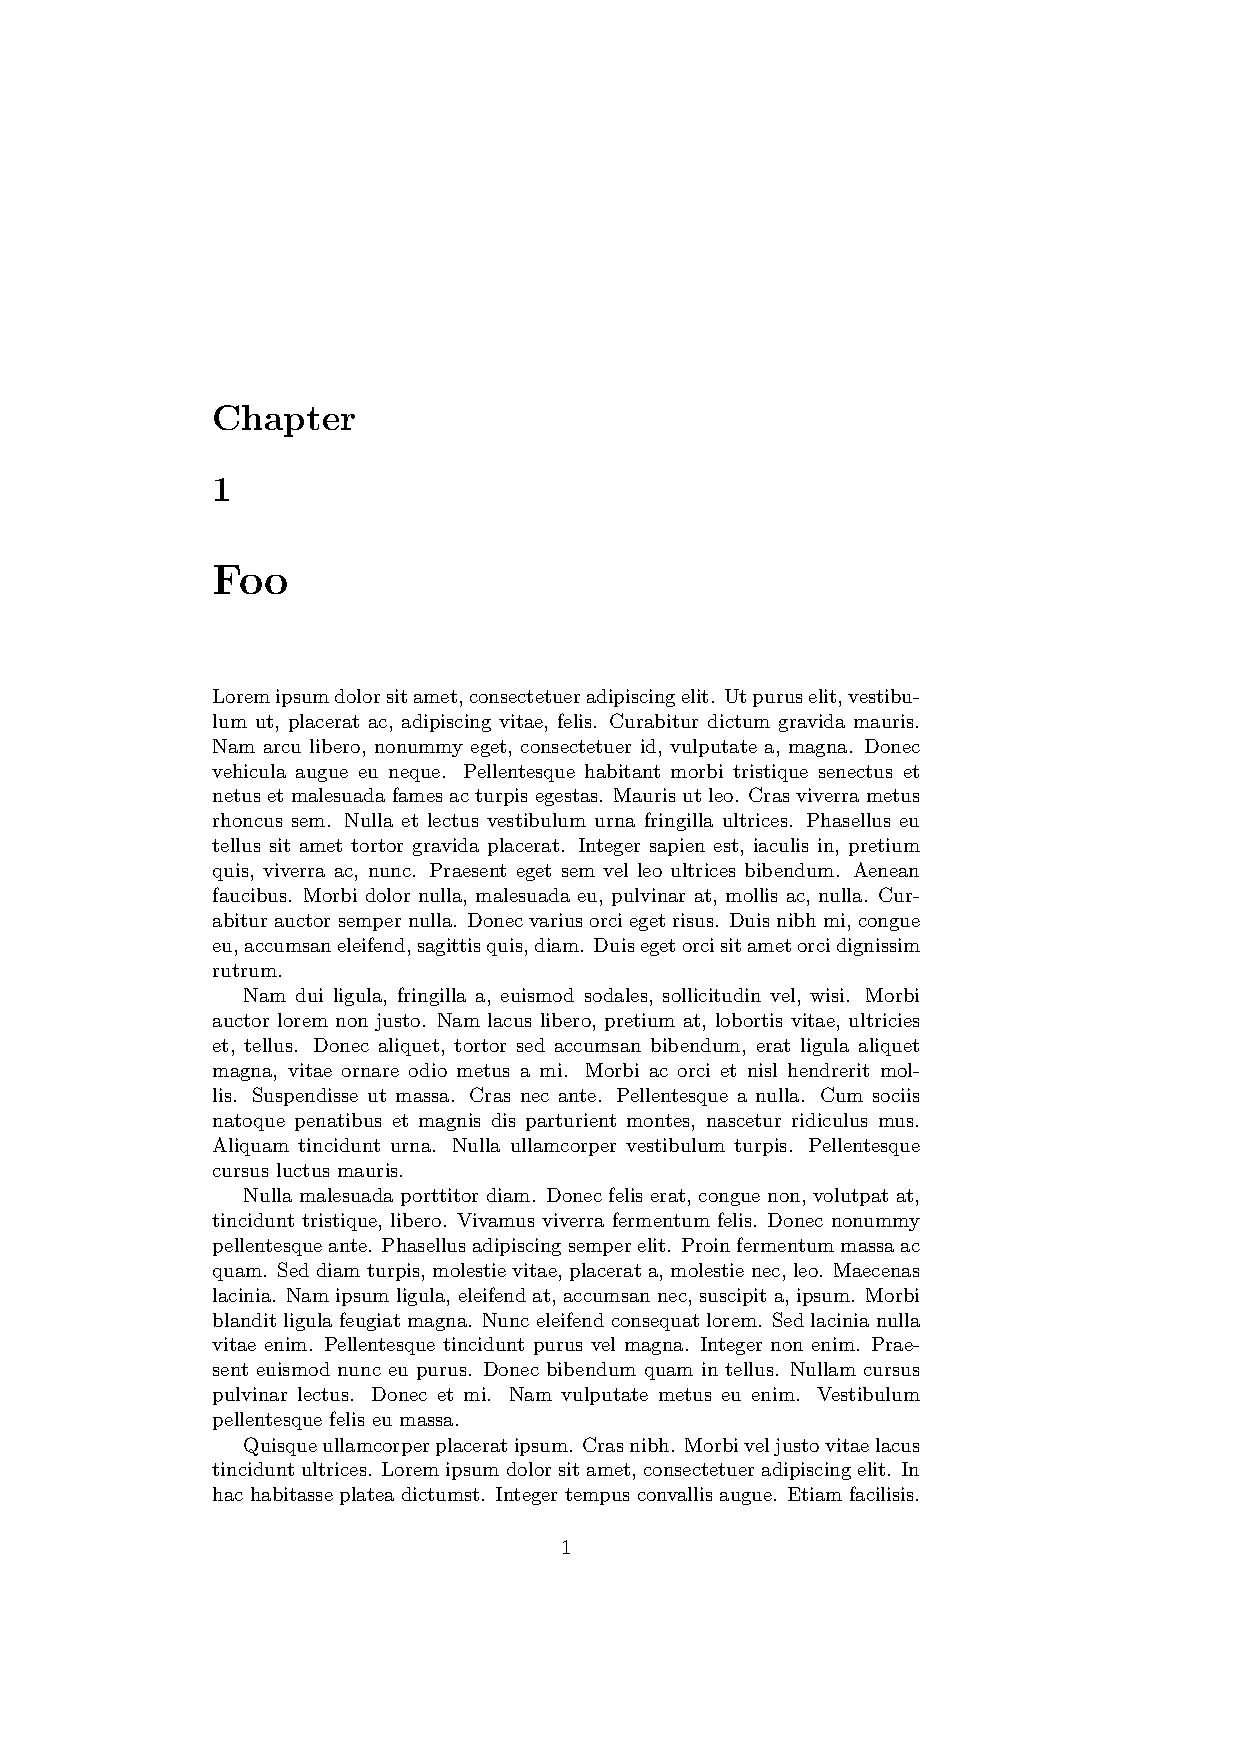
\includegraphics[frame,page=1,width=\linewidth]{examples/chapternamenum}
    \end{column}
  \end{columns}
\end{frame}

\begin{frame}[fragile]
  {\texttt{\tbs printchapternum}과 \texttt{\tbs chapnumfont} 분석}
  \ltxverb/\printchaptername/과 \ltxverb/\chapnumfont/의 관계처럼
  \ltxverb/\printchapternum/은 챕터 번호를, 사용되는 글꼴은
  \ltxverb/\chapnumfont/로 지정한다.
  \ltxverb/\chapnumfont/의 기본값은 \ltxverb/\chapnamefont/와 같은
  \ltxverb/\bfseries\huge/이다.
\end{frame}

\begin{frame}[fragile]
  {\texttt{\tbs printchapternum} 및 \texttt{\tbs chapnumfont} 예시}
  \begin{columns}
    \begin{column}{0.6\textwidth}
      \begin{latexcode}
        \renewcommand*{\printchapternum}{%
          \chapnumfont\thechapter}
        \renewcommand*{\chapnumfont}{\slshape\Huge}
      \end{latexcode}
    \end{column}

    \begin{column}{0.4\textwidth}
      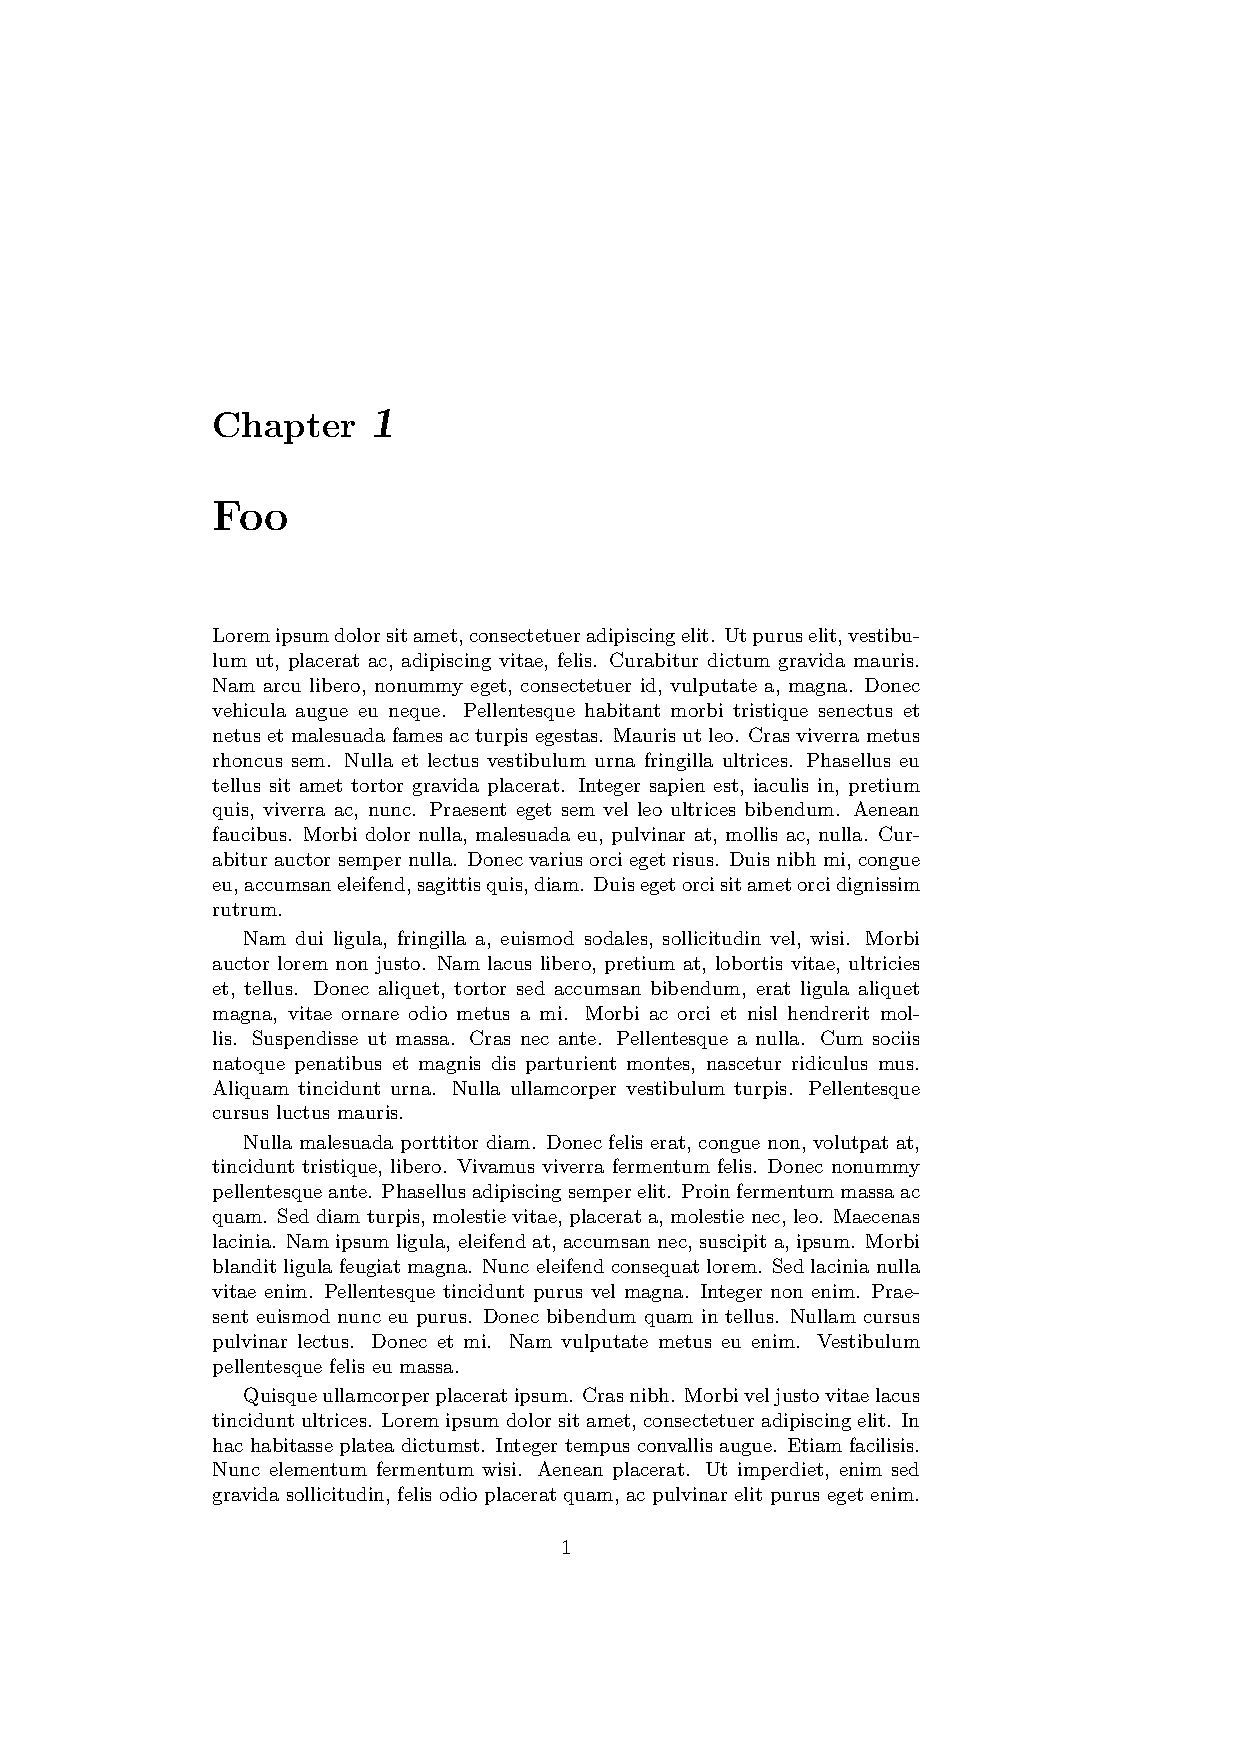
\includegraphics[frame,page=1,width=\linewidth]{examples/printchapternum}
    \end{column}
  \end{columns}
\end{frame}

\begin{frame}[fragile]
  {\texttt{\tbs printchaptertitle}과 \texttt{\tbs chaptitlefont} 분석}
  이전과 마찬가지로 \ltxverb/\printchaptertitle/은 챕터 번호를, 사용되는 글꼴은
  \ltxverb/\chaptitlefont/로 지정한다.
  \ltxverb/\chaptitlefont/의 기본값은 \ltxverb/\bfseries\Huge/이다.
\end{frame}

\begin{frame}[fragile]
  {\texttt{\tbs printchaptertitle}과 \texttt{\tbs chaptitlefont} 예시}
  \begin{columns}
    \begin{column}{0.6\textwidth}
      \begin{latexcode}
        \renewcommand*{\chaptitlefont}{%
          \normalfont\scshape\Huge}
        \renewcommand*{\printchaptertitle}[1]{%
          \chaptitlefont #1}
      \end{latexcode}
    \end{column}

    \begin{column}{0.4\textwidth}
      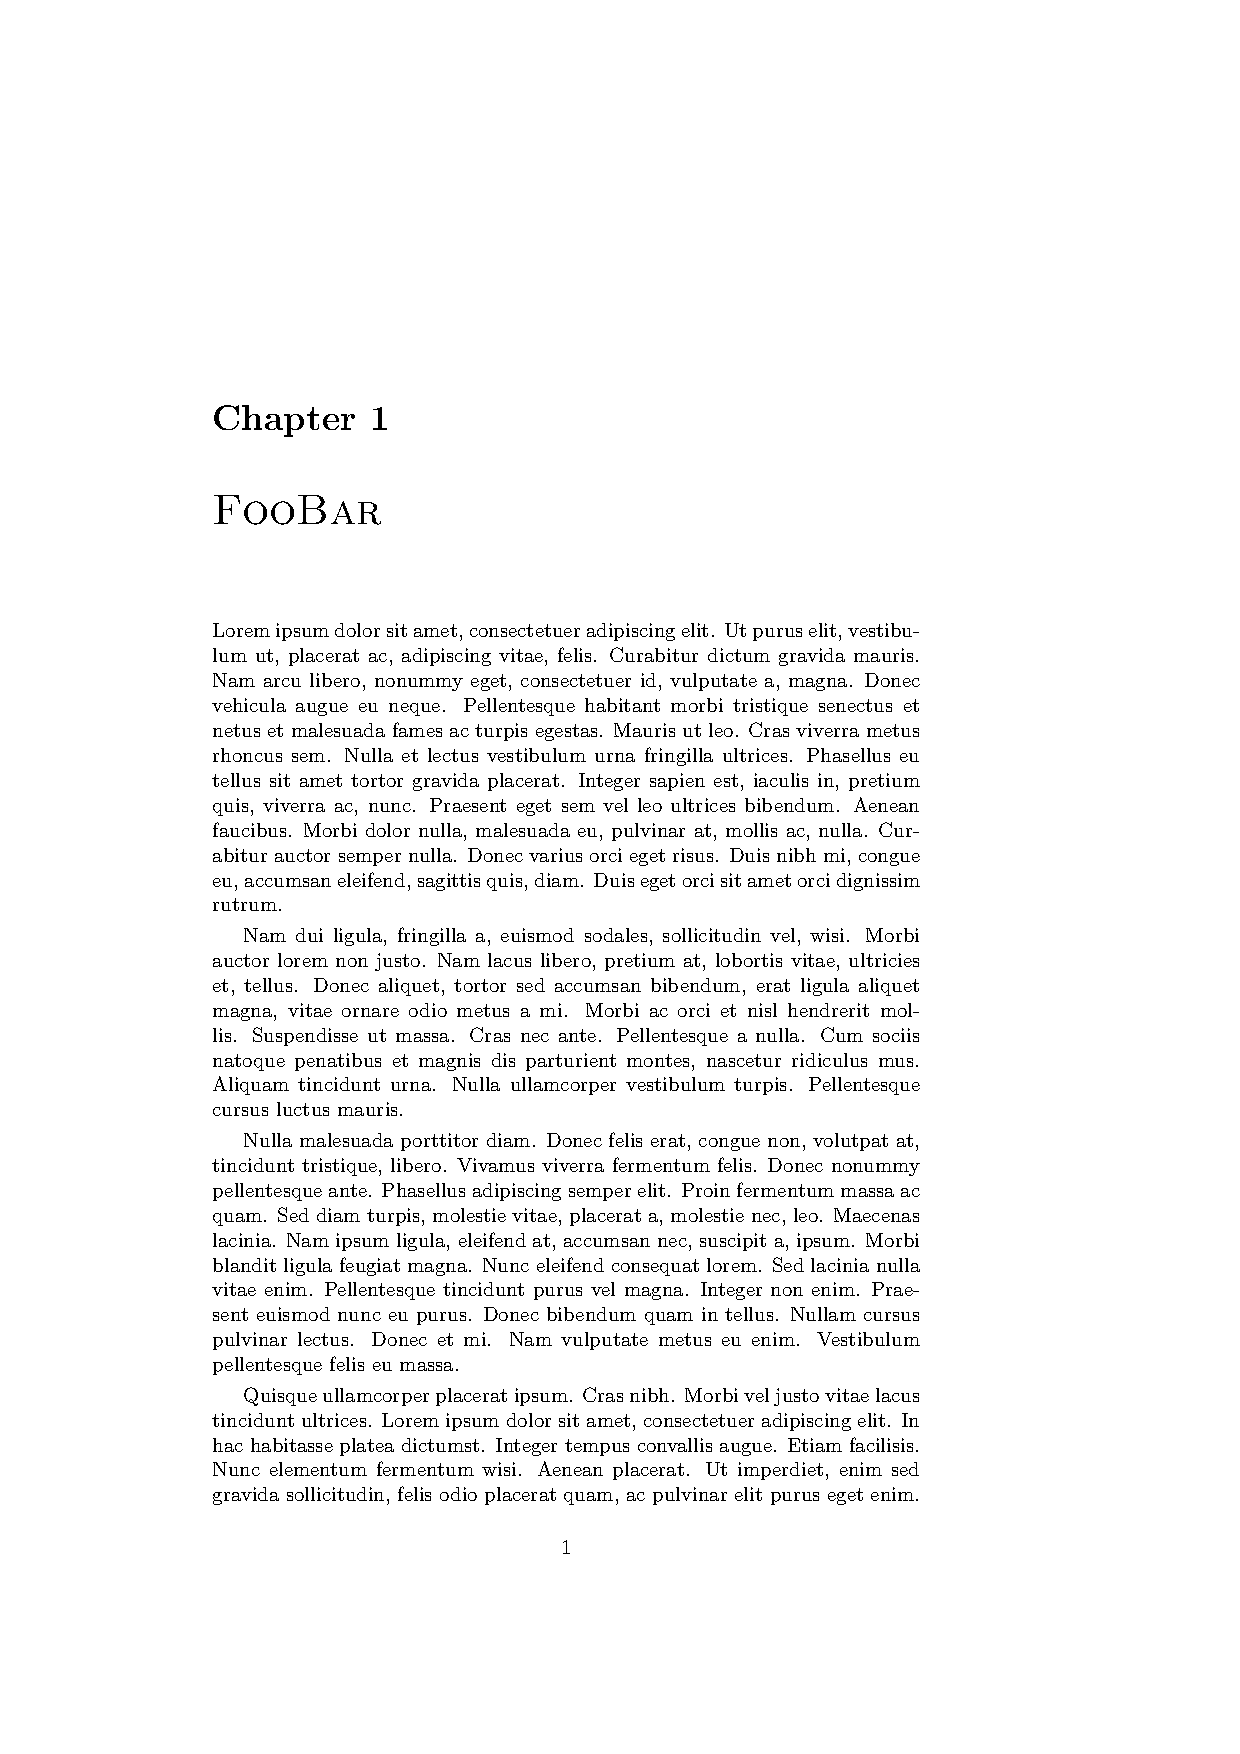
\includegraphics[frame,page=1,width=\linewidth]{examples/printchaptertitle}
    \end{column}
  \end{columns}
\end{frame}

\begin{frame}{Summary}
  \begin{center}
    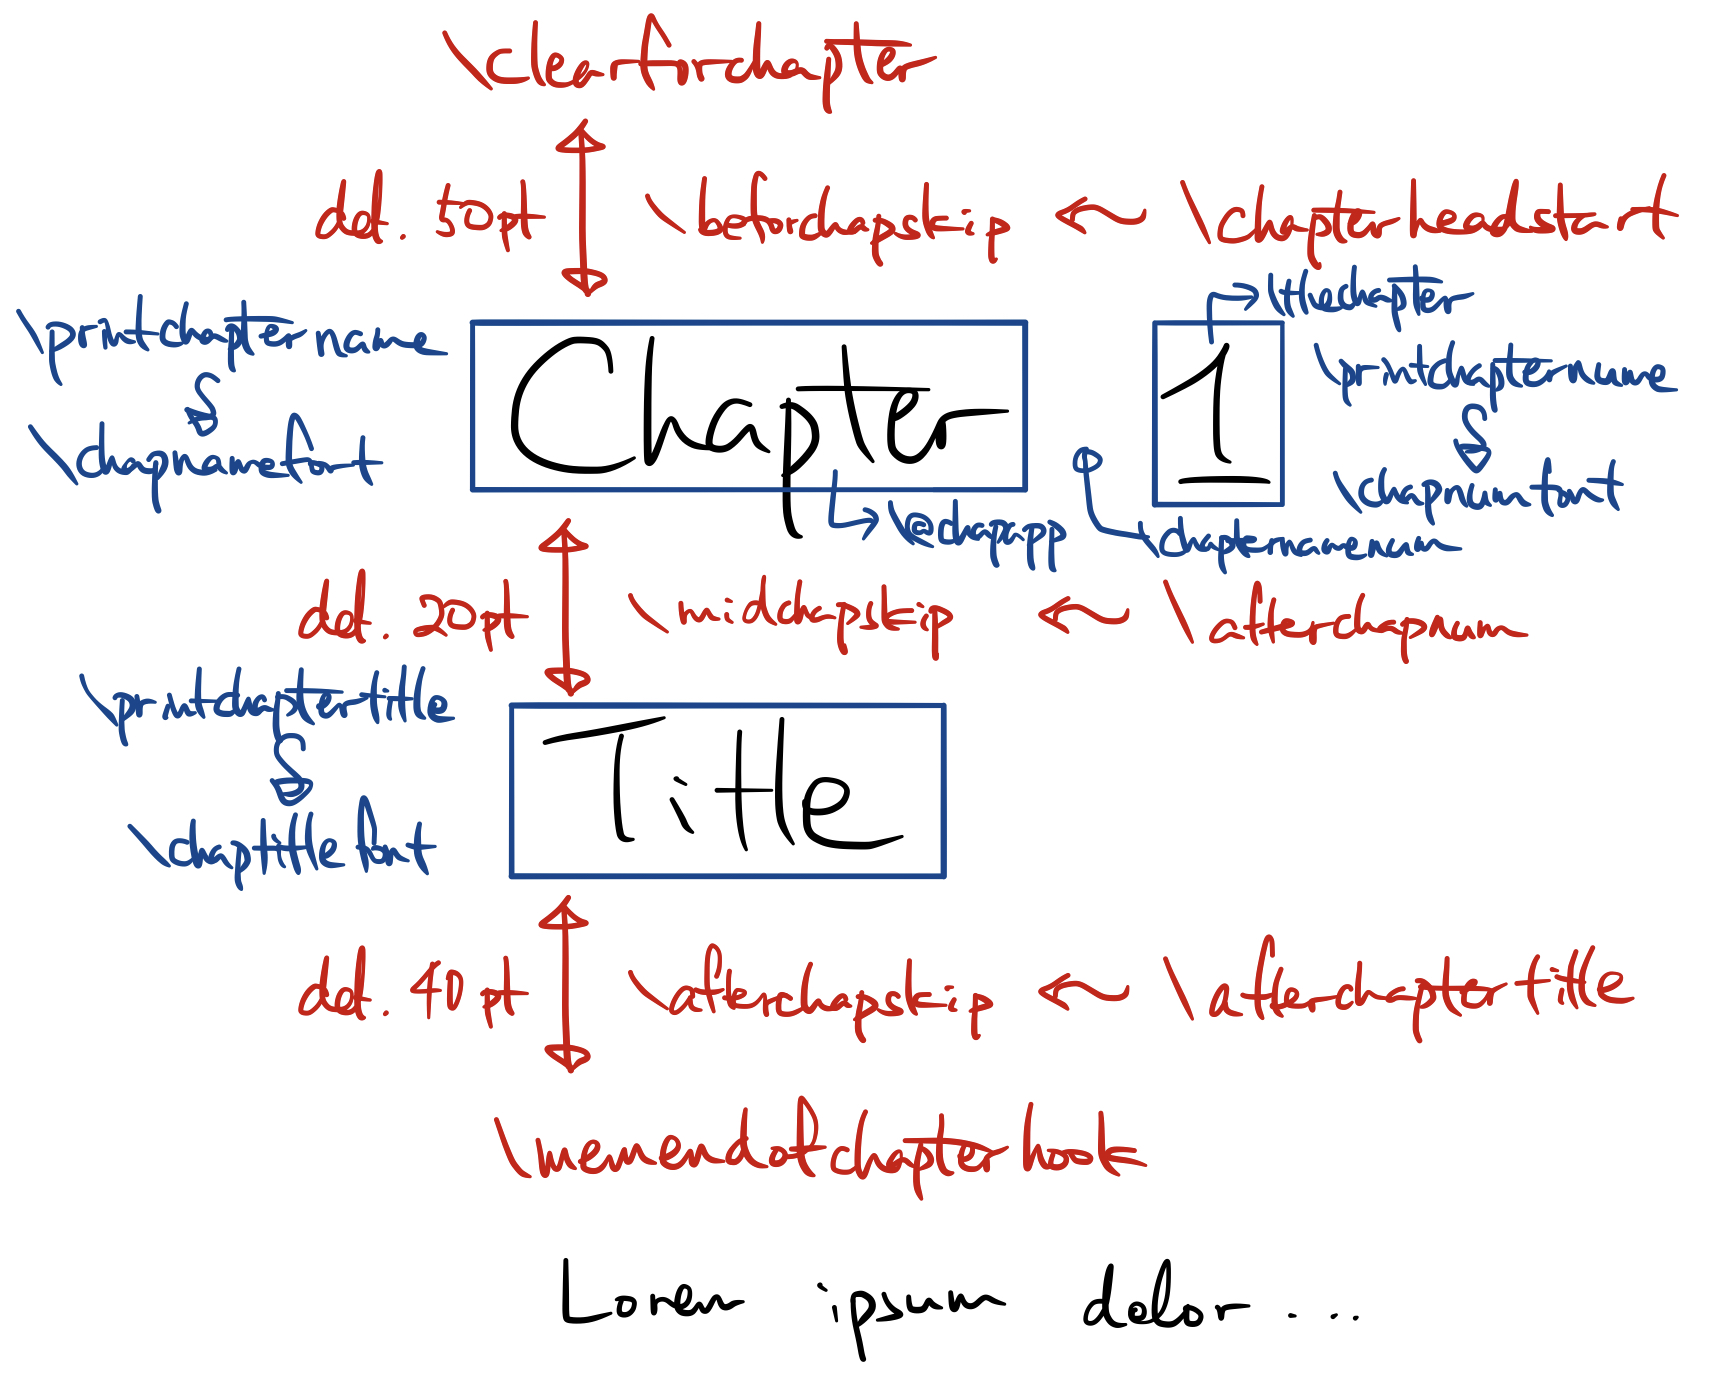
\includegraphics[width=0.8\textwidth]{summary}
  \end{center}
\end{frame}

\section{Case Study}

\begin{frame}[fragile]{Introduction to Electrodynamics (Griffiths)}
  \begin{columns}
    \begin{column}{0.5\textwidth}
      엊그제 전자기학 시험을 봤습니다$\ldots$
      \pause

      Griffiths의 Introduction to Electrodynamics 교재의 chapter style을
      모방하며 위의 명령어들을 활용해봅시다.
    \end{column}
    \begin{column}{0.5\textwidth}
      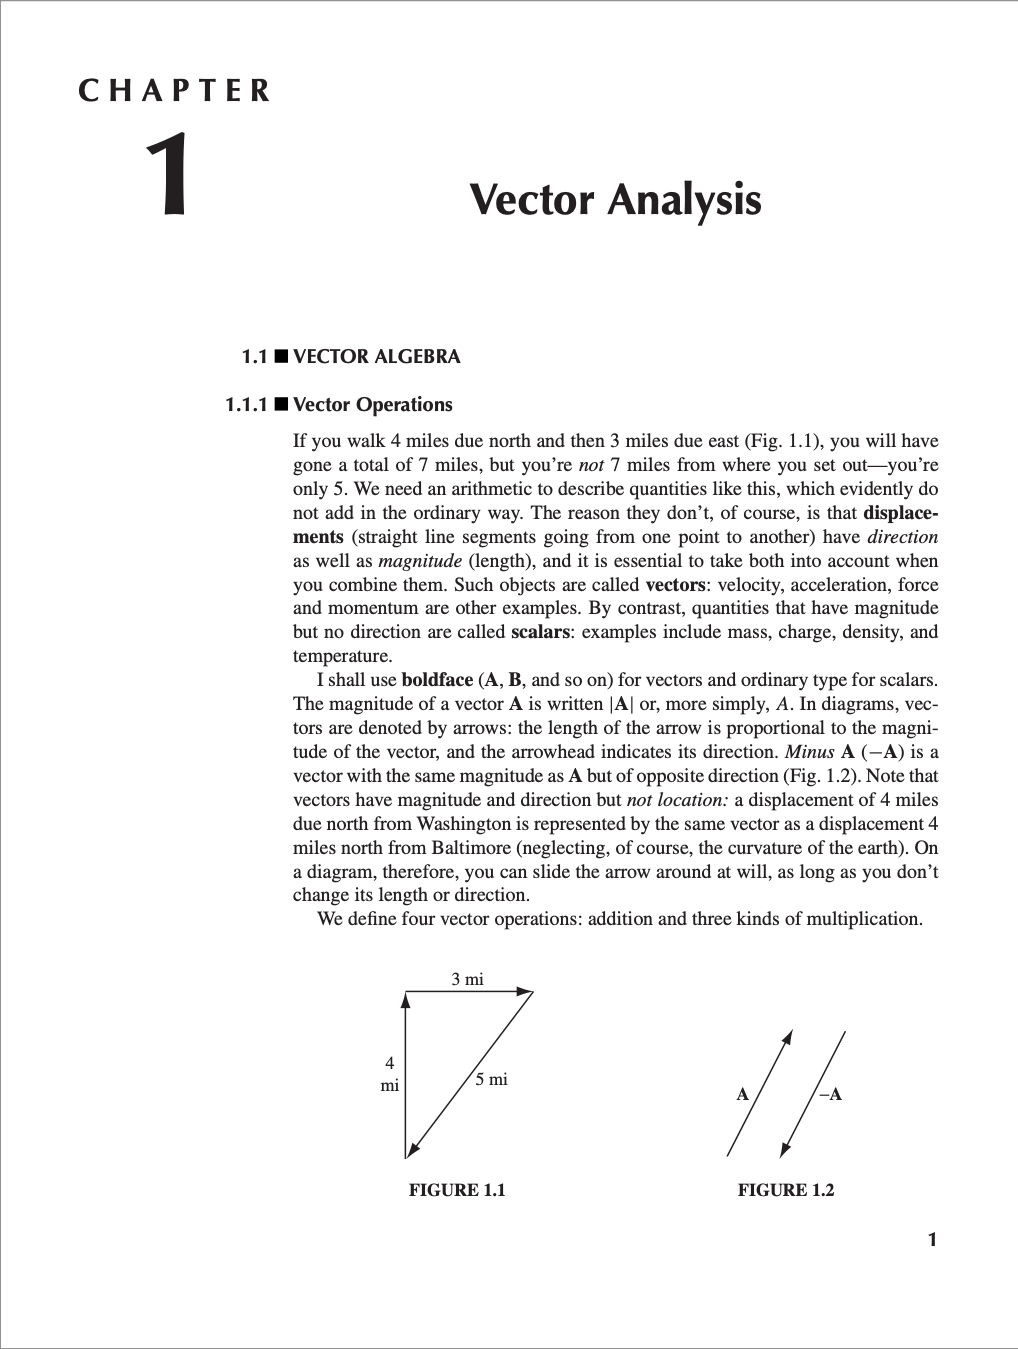
\includegraphics[frame,width=\linewidth]{examples/griffiths-sample}
    \end{column}
  \end{columns}
\end{frame}

\begin{frame}[fragile]{페이지 레이아웃 및 글꼴 설정 (참고)}
  \begin{columns}
    \begin{column}{0.5\textwidth}
      \begin{latexcode}
        \documentclass[openany]{memoir}

        % Page layout settings
        \setstocksize{237mm}{179mm}
        \settrimmedsize{\stockheight}{\stockwidth}{*}
        \setlrmarginsandblock{146pt}{39pt}{*}
        \setulmarginsandblock{60pt}{76pt}{*}
        \setheaderspaces{*}{13pt}{*}
        \checkandfixthelayout
        \setlength{\evensidemargin}{\oddsidemargin}

        % Font settings
        \usepackage{amsmath}
        \usepackage[(생략)]{mtpro2}
        \usepackage[no-math]{fontspec}
        \setmainfont{Times New Roman}
        \newfontfamily\optimafont{Optima}
      \end{latexcode}
    \end{column}
    \begin{column}{0.5\textwidth}
      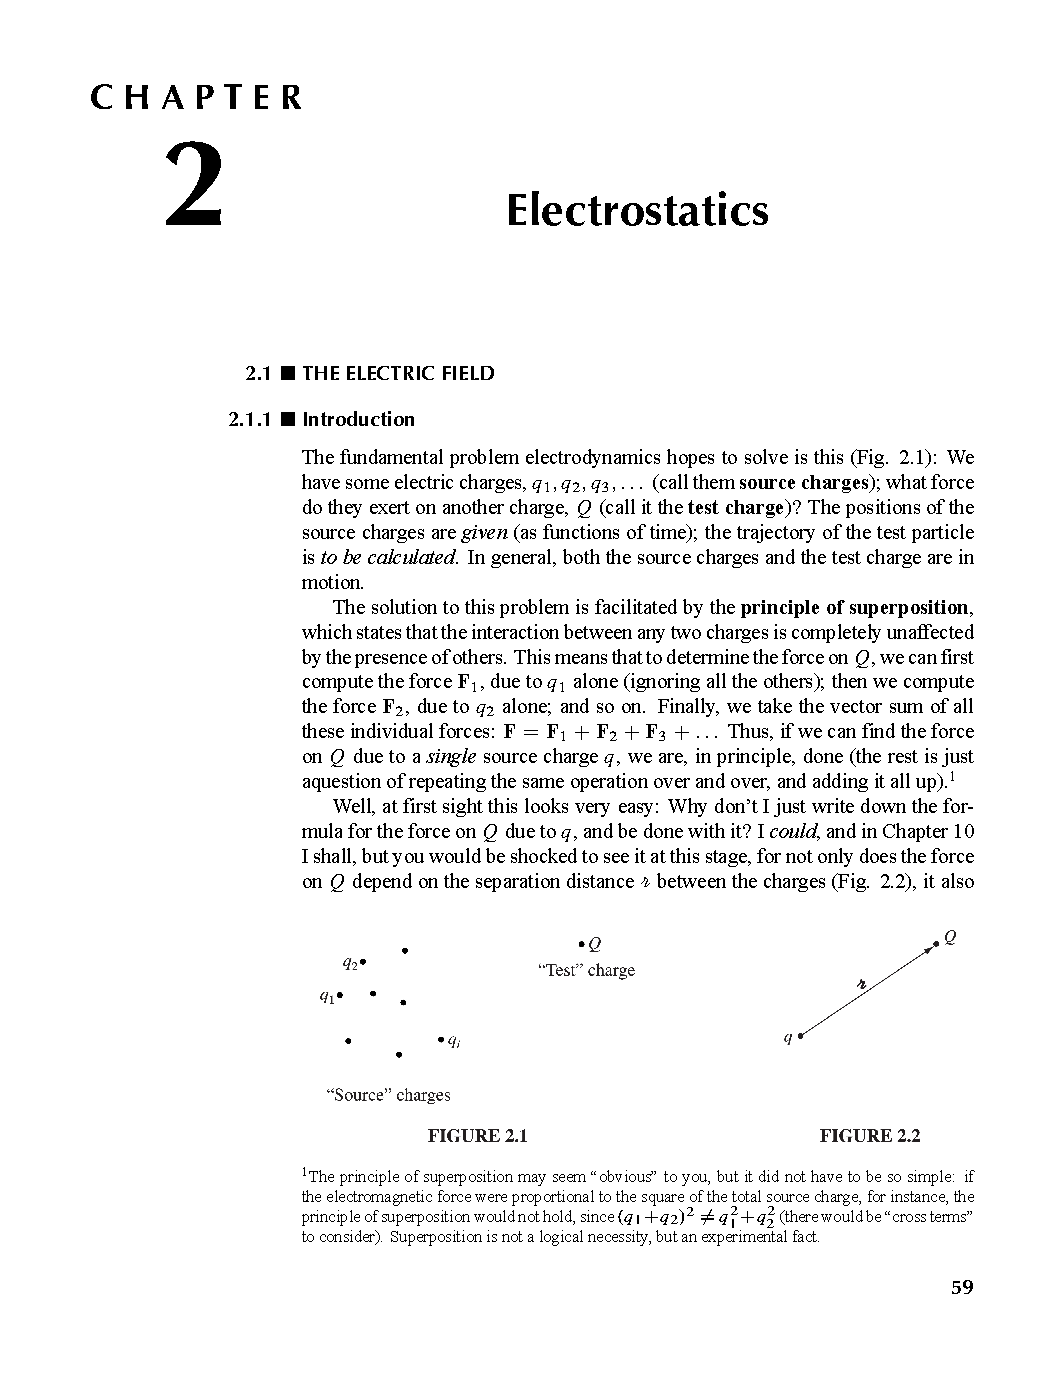
\includegraphics[frame,page=1,width=\linewidth]{examples/griffiths-clone}
    \end{column}
  \end{columns}
\end{frame}

\begin{frame}[fragile]{페이지 스타일 설정 (참고)}
  \begin{columns}
    \begin{column}{0.5\textwidth}
      \begin{latexcode}
        \newcommand*{\shiftleft}[2]{%
          \makebox[0pt][r]{%
            \makebox[#1][l]{#2}}}
        % Pagestyle settings
        (생략)
        % 챕터가 나오는 쪽에 대한 페이지 스타일
        \makepagestyle{gchapter}
        % 쪽 번호가 왼쪽에 올 경우에는 텍스트보다 왼쪽으로 107pt 옮겨서 표시
        \makeevenfoot{gchapter}{%
          \optimafont\shiftleft{107pt}{%
            \bfseries\thepage}}{}{}
        \makeoddfoot{gchapter}{}{}{%
          \optimafont\bfseries\thepage}
      \end{latexcode}
    \end{column}
    \begin{column}{0.5\textwidth}
      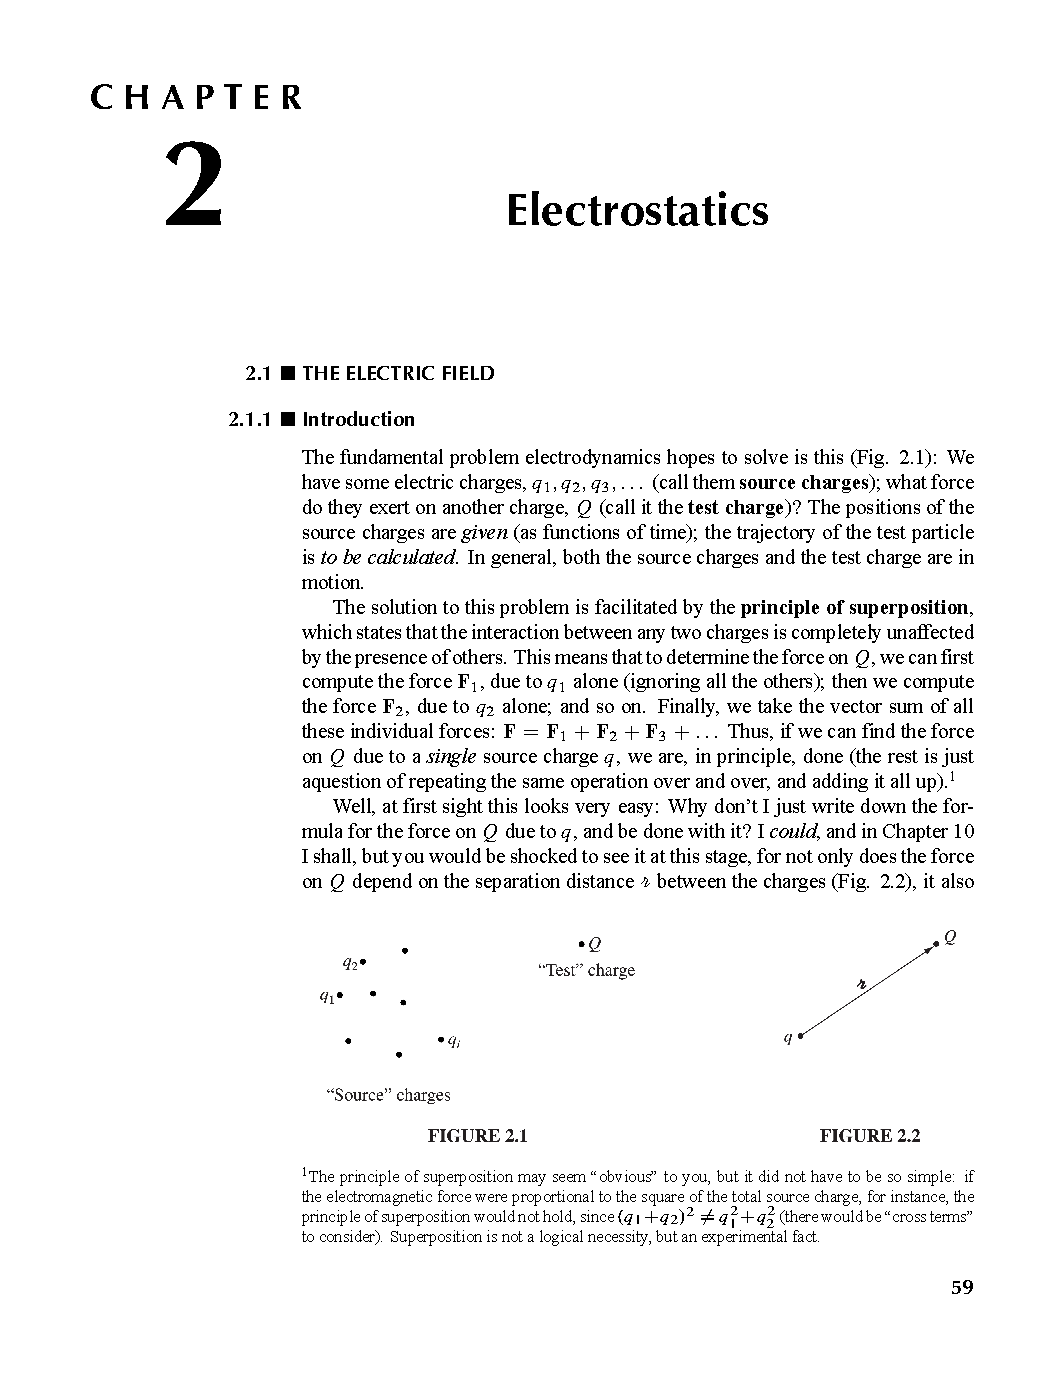
\includegraphics[frame,page=1,width=\linewidth]{examples/griffiths-clone}
    \end{column}
  \end{columns}
\end{frame}

\begin{frame}[fragile]{챕터 스타일 설정 1}
  \begin{columns}
    \begin{column}{0.5\textwidth}
      \begin{latexcode}
        % Chapterstyle settings
        \makeatletter
        \newlength{\chapappwidth}
        \makechapterstyle{griffiths}{%
          % 기본 챕터 스타일에서 시작
          \chapterstyle{default}
          \setlength\beforechapskip{-42pt}
          \renewcommand*{\afterchapternum}{%
            \qquad}
          \setlength\afterchapskip{63pt}
      \end{latexcode}
    \end{column}
    \begin{column}{0.5\textwidth}
      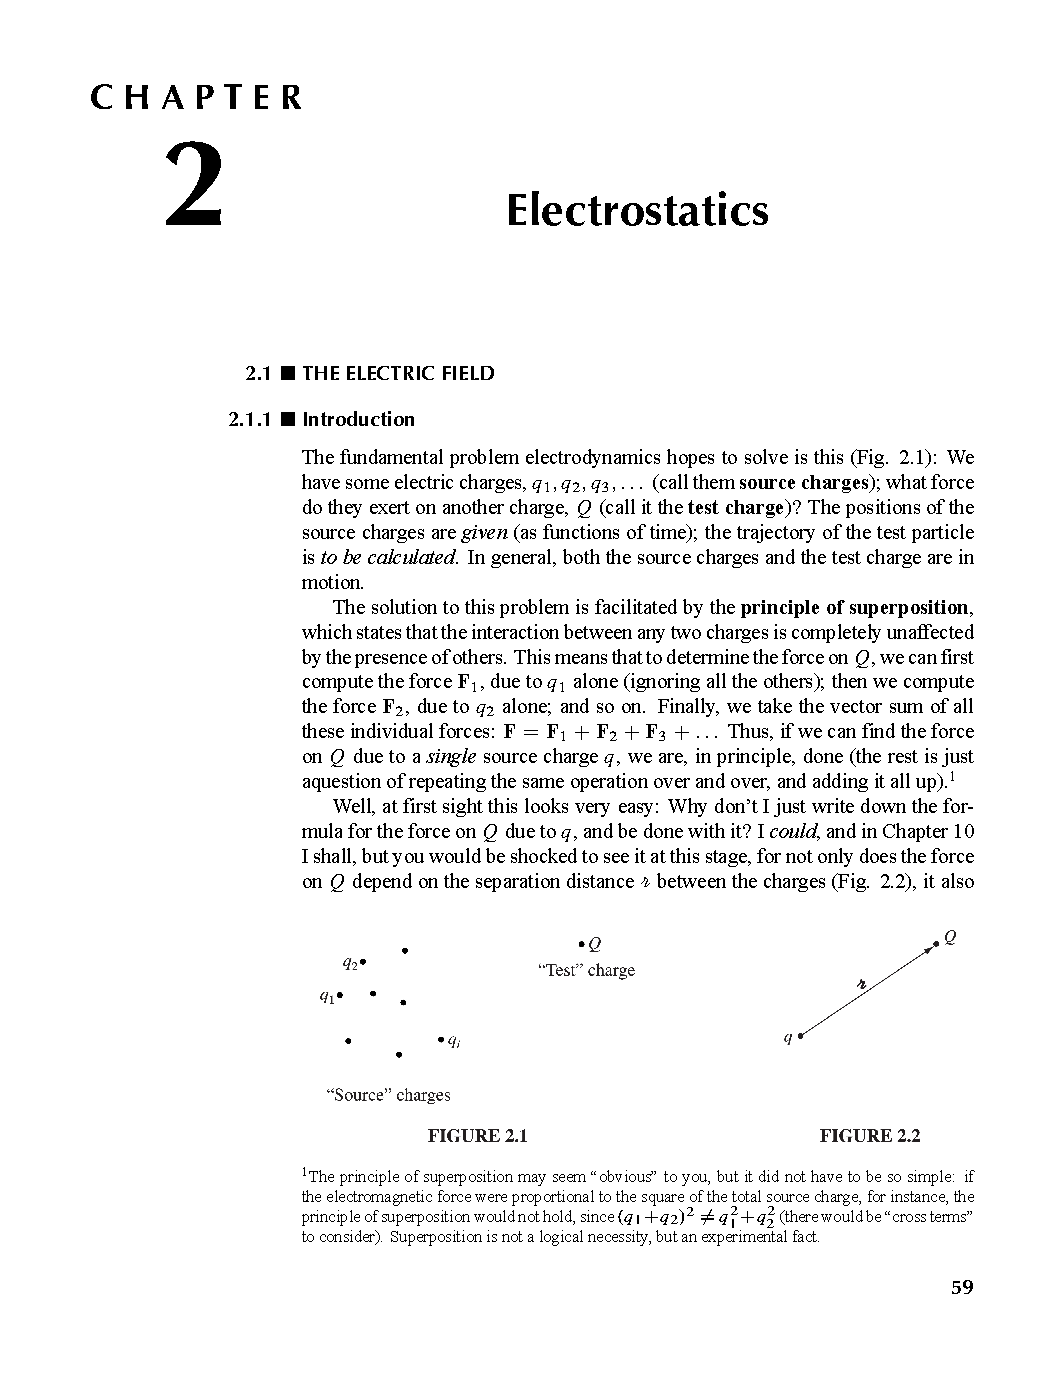
\includegraphics[frame,page=1,width=\linewidth]{examples/griffiths-clone}
    \end{column}
  \end{columns}
\end{frame}

\begin{frame}[fragile]{챕터 스타일 설정 2}
  \begin{columns}
    \begin{column}{0.5\textwidth}
      \begin{latexcode}
        \renewcommand*{\chapnamefont}{%
          \optimafont\bfseries%
          \addfontfeatures{LetterSpace=26}%
          \huge}
        \def\chaptertext{\chapnamefont%
          \MakeUppercase{\@chapapp}}
        % CHAPTER의 너비를 저장
        \settowidth{\chapappwidth}{\chaptertext}
        \renewcommand*{\printchaptername}{%
          % 왼쪽 여백을 줄임
          \begin{adjustwidth}{%
            -\chapappwidth}{}
            \chaptertext
          \end{adjustwidth}}
        \renewcommand*{\chapternamenum}{%
          \vskip 12pt}
        \renewcommand*{\chapnumfont}{%
          \optimafont\bfseries%
          \fontsize{60}{60}\selectfont}
      \end{latexcode}
    \end{column}
    \begin{column}{0.5\textwidth}
      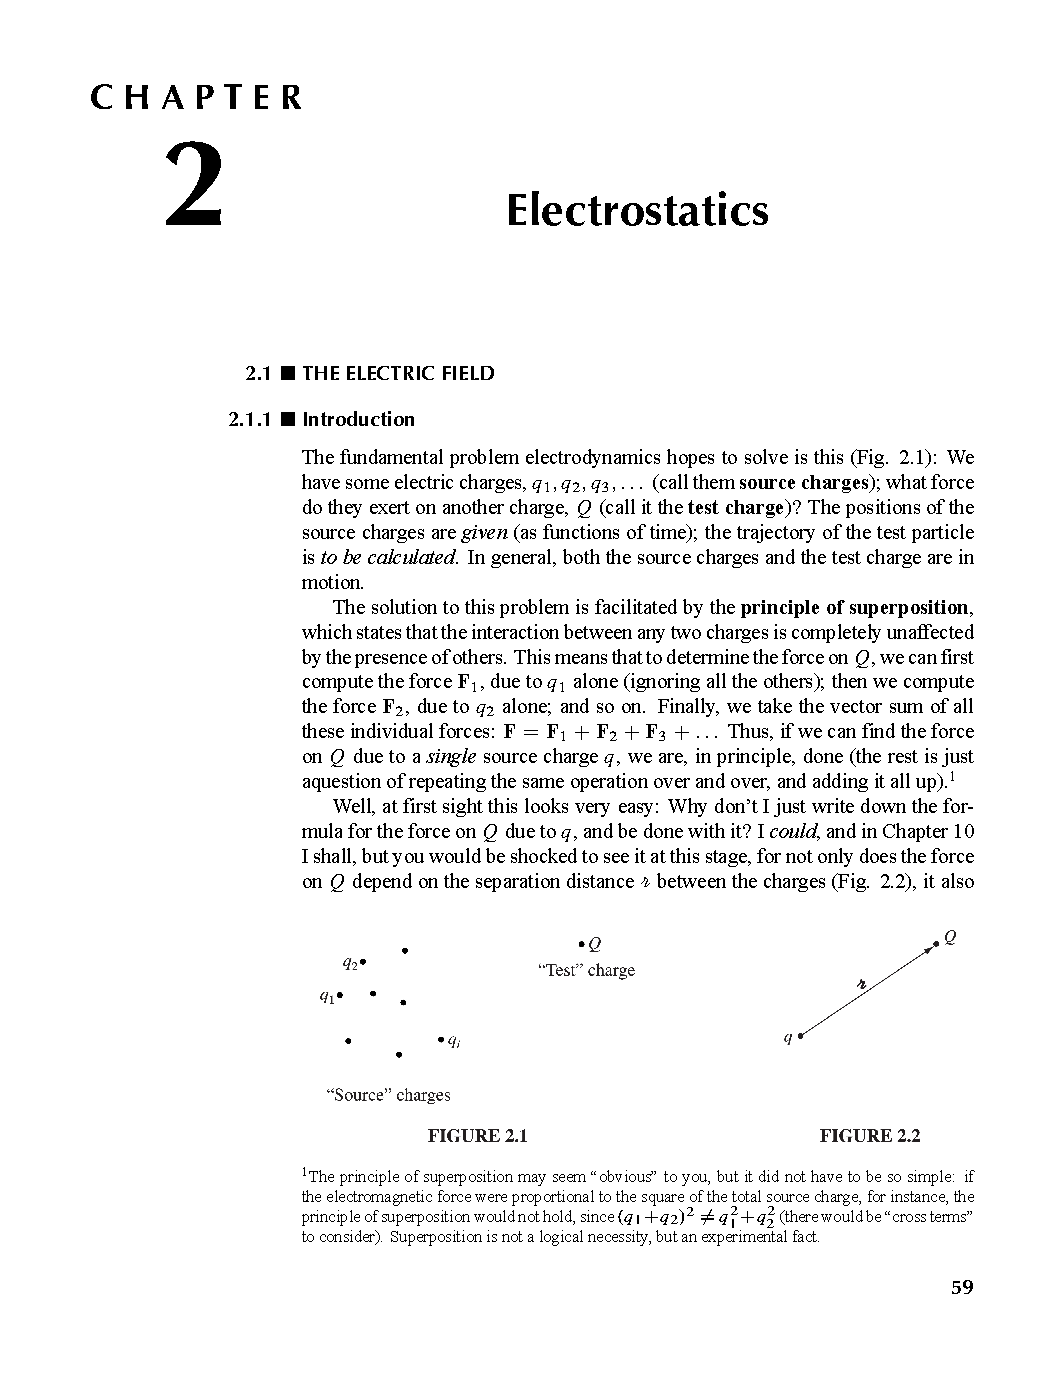
\includegraphics[frame,page=1,width=\linewidth]{examples/griffiths-clone}
    \end{column}
  \end{columns}
\end{frame}

\begin{frame}[fragile]{챕터 스타일 설정 3}
  \begin{columns}
    \begin{column}{0.5\textwidth}
      \begin{latexcode}
        % 챕터 번호는 \printchaptertitle에서 같이 출력하도록 지정
        \renewcommand*{\printchapternum}{}
        \renewcommand*{\chaptitlefont}{%
          \optimafont\bfseries%
          \fontsize{22}{22}\selectfont}
        \renewcommand*{%
          \printchaptertitle}[1]{%
          \begin{adjustwidth}{%
            -\chapappwidth}{}
            \makebox[\chapappwidth][c]{%
              \chapnumfont\thechapter}%
            \makebox[\dimexpr\linewidth-\chapappwidth\relax][c]{%
              \chaptitlefont ##1}
          \end{adjustwidth}}}
        \makeatother
        % 챕터 쪽의 페이지 스타일 지정
        \renewcommand*{\memendofchapterhook}{%
          \thispagestyle{gchapter}}
      \end{latexcode}
    \end{column}
    \begin{column}{0.5\textwidth}
      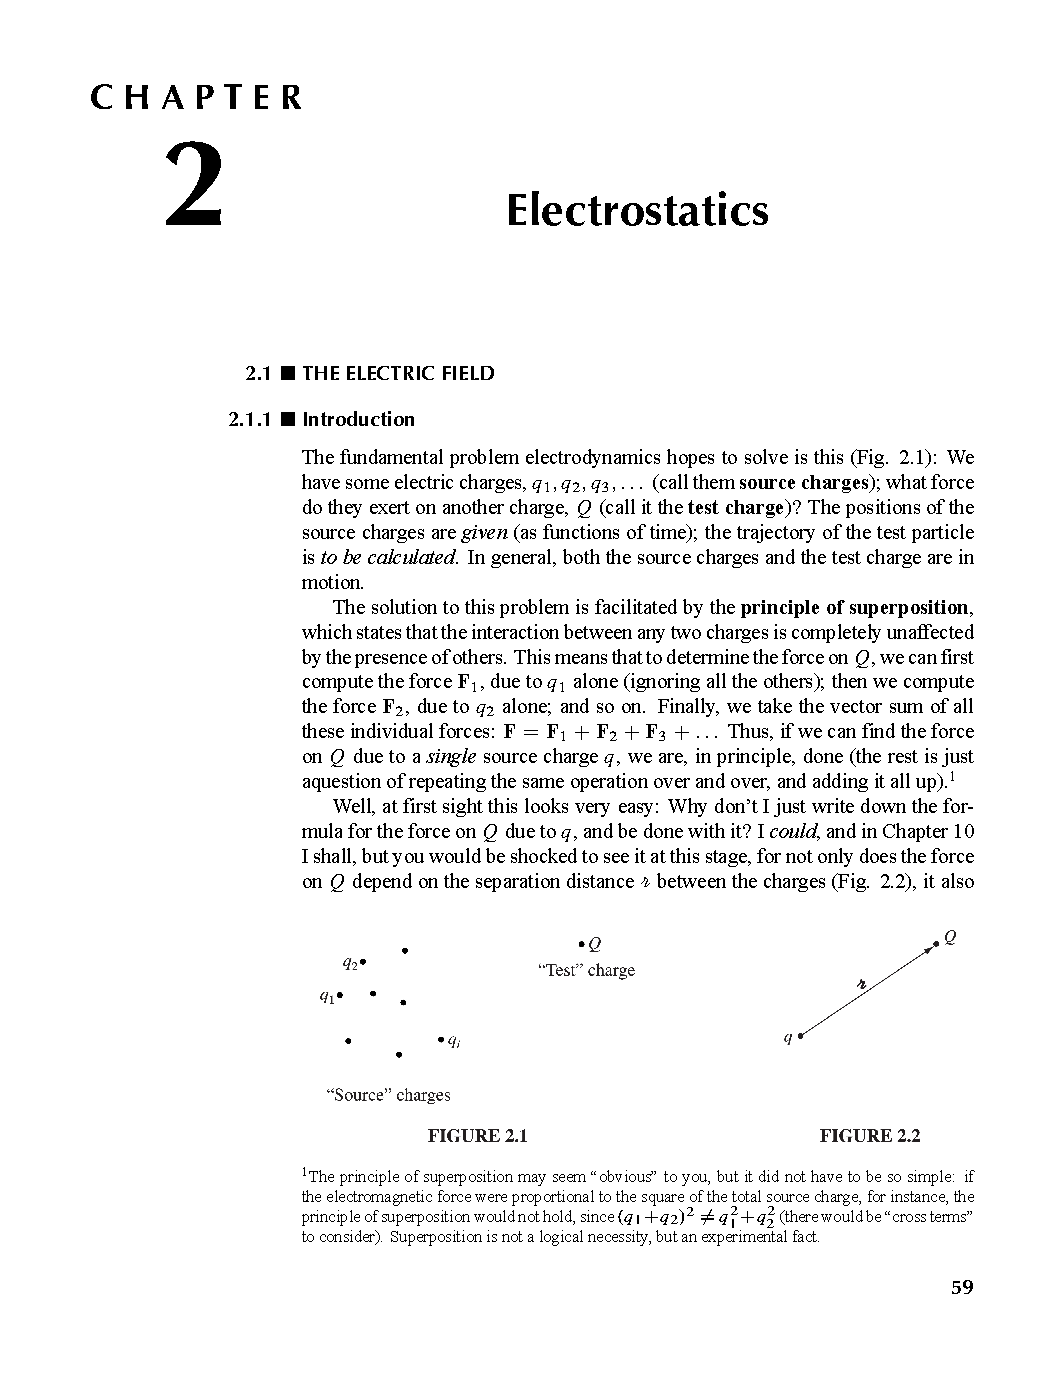
\includegraphics[frame,page=1,width=\linewidth]{examples/griffiths-clone}
    \end{column}
  \end{columns}
\end{frame}

\begin{frame}[fragile]{기타 서식 설정}
  \begin{columns}
    \begin{column}{0.5\textwidth}
      \begin{latexcode}
        % Sectionstyle settings
        \setsecnumdepth{subsection}
        \maxsecnumdepth{subsection}

        \setsecnumformat{\llap{%
          \csname the#1\endcsname\ $\blacksquare$\ }}
        \setsecheadstyle{%
          \optimafont\bfseries\MakeUppercase}
        \setsubsecheadstyle{\optimafont\bfseries}

        % Footnote settings
        \setlength{\footmarkwidth}{0pt}
        \setlength{\footmarksep}{0pt}
        \let\oldfootnoterule\footnoterule
        \renewcommand*{\footnoterule}{}
      \end{latexcode}
    \end{column}
    \begin{column}{0.5\textwidth}
      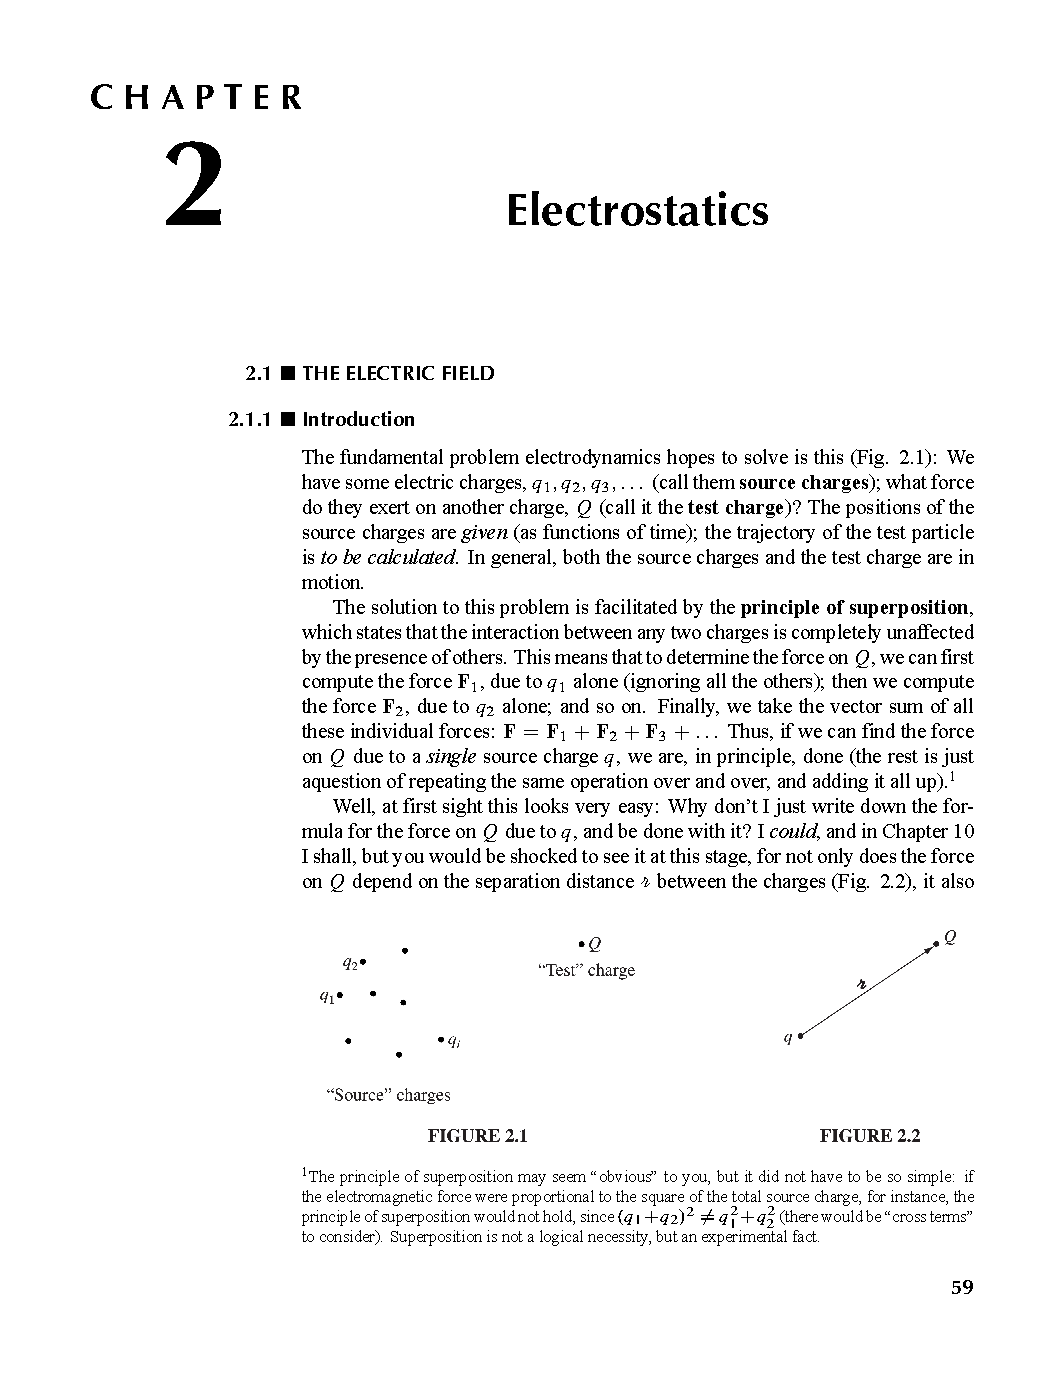
\includegraphics[frame,page=1,width=\linewidth]{examples/griffiths-clone}
    \end{column}
  \end{columns}
\end{frame}

\begin{frame}{마무리}
  \pause
  \centering 감사합니다.
\end{frame}

\begin{frame}{부록}
  본 발표 자료는
  \url{https://github.com/Zeta611/chapterstyle-latex-workshop-2019}에서 소스와
  함께 보실 수 있으며, case study에서 살펴본 챕터 스타일은
  \url{https://github.com/Zeta611/griffiths-clone/}에서 보실 수 있습니다.

  또한 본 주제를 포함한 Memoir에 관한 모든 내용은 \texttt{texdoc memoir}을
  터미널에 입력하시면 읽어보실 수 있습니다.

  \begin{center}
    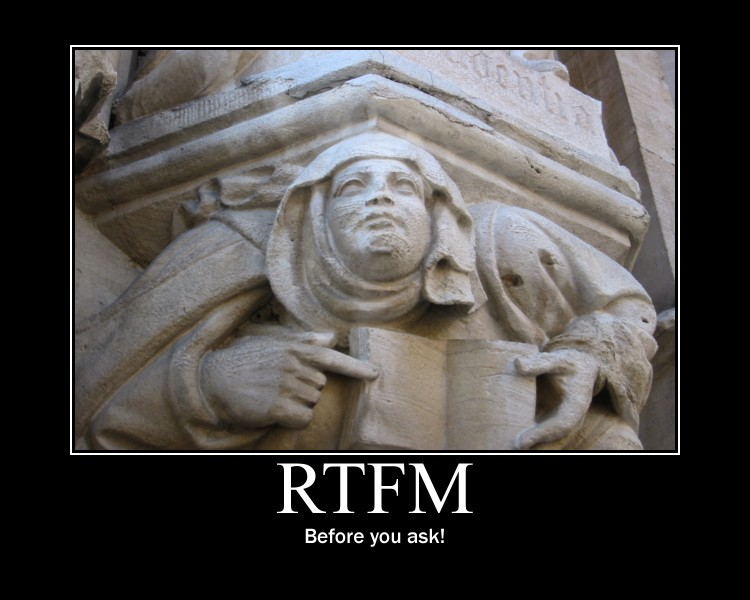
\includegraphics[width=0.4\linewidth]{rtfm}
  \end{center}
\end{frame}
\end{document}
